\chapter{O Método dos Elementos Finitos}

\begin{quote}
    "As far as the laws of mathematics refer to reality, they are not certain; and as far as they are certain, they do not refer to reality." (Albert Einstein)
\end{quote}

O método dos elementos finitos (MEF) é um procedimento numérico utilizada para encontrar soluções de equações que modelam a natureza. É amplamente utilizado na simulação de fenômenos físicos, como mecânica dos sólidos, transferência de calor, eletromagnetismo e muitos outros. \cite{Onate}

A abordagem do MEF envolve a subdivisão de uma estrutura ou domínio contínuo em pequenos elementos geométricos finitos, definidos por nós, caracterizados por suas propriedades físicas e geométricas, em que são aplicadas as equações governantes do problema, cujo campo é aproximado, dentro de cada um, por meio de funções de interpolação, que vão discretizar o campo sobre os valores nodais. Em seguida, essas equações aproximadas são montadas, justapondo os elementos, em um sistema global, levando em consideração as condições de contorno e as restrições do problema. \cite{LIU}

Em suma, o método de elementos finitos segue o seguinte procedimento, de acordo com \citeshort{Onate}:

\begin{enumerate}
    \item definição do domínio, e das condições de contorno;
    \item discretização do domínio em uma malha formada por nós que constituem os elemento;
    \item aplicação das equações de governo sobre cada elemento, formando um sistema local de rigidez;
    \item montagem dessas equações em um único grande sistema global;
    \item resolução do sistema, encontrando os valores nodais do campo.
\end{enumerate}

Na análise estrutural aqui abordada, o objetivo da aplicação do MEF é determinar o deslocamento de um sólido em equilíbrio sujeito a carregamentos e restrições, dentro do regime elástico modelado pela Lei de Hooke, utilizando funções de interpolações lineares em elementos triangulares (na análise 2D: EPT ou EPD) e tetraédricos (na análise 3D). Para tanto, resolver um sistema da forma

\begin{equation}
    \bm{K} \bm{U} = \bm{F},
    \label{eq:sistema_global}
\end{equation}
em que $\bm{K}$ é a matriz de rigidez global, $\bm{U}$ é o vetor de deslocamentos nodais, e $\bm{F}$ é o vetor de forças nodais.

Deste modo, convém definir os termos e símbolos dessas entidades matemáticas. Seja um corpo $\mathcal{B}$, definido por uma geometria sobre o domínio $\Omega$, que é repartido em pequenos elementos, de domínio $\Omega^{(e)}$, cuja fronteira se denomina $\partial\Omega^{(e)}$. A figura \ref{fig:dominio_triangulo} mostra um domínio bidimensional $\Omega$ discretizado em elementos triangulares, cujos nós são representados por $i, j$ e $k$. Quando uma entidade é definida sobre um elemento, ela é representada por um superescrito $(e)$, como por exemplo o deslocamento $\bm{\varphi}^{(e)}$ sobre o elemento $e$.

Seguindo \citeshort{LOGAN}, neste capítulo aborda-se como
\begin{enumerate}
    \item selecionar as funções de interpolação;
    \item definir as relações de tensão-deformação-deslocamento;
    \item derivar a forma da matriz de rigidez;
    \item montar o sistema global e introduzir as condições de contorno.
\end{enumerate}

\begin{figure}
	\centering
    \caption{Domínio discretizado em elementos triangulares.}
    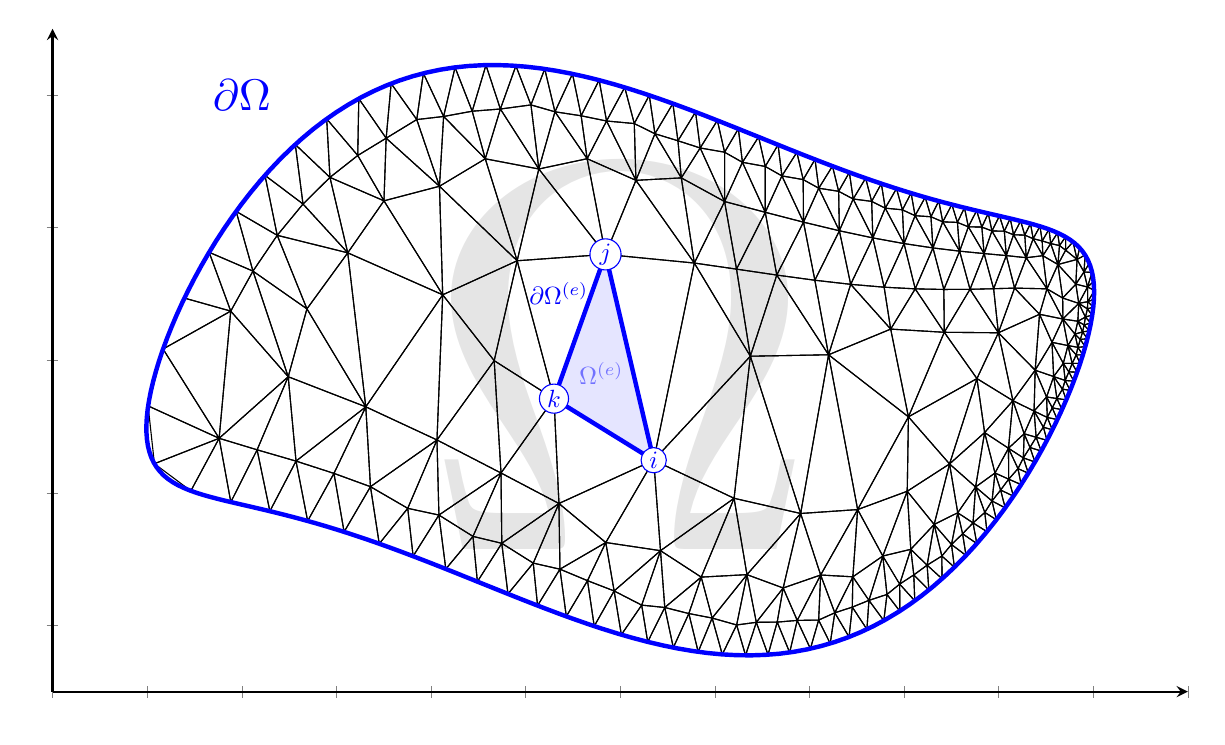
\begin{tikzpicture}
        \begin{axis}[
                xmin = -6, xmax = 6,
                ymin = -2.5, ymax = 2.5, 
                height = 10 cm, width = 16 cm,
                axis lines = left,
                xticklabels = {,,},
                yticklabels = {,,},
                axis line style = thick
            ]
                \draw (4.957784,0.2214301) -- (4.971856,0.2809534) -- (4.903003,0.2658061) -- cycle;\draw (4.971856,0.2809534) -- (4.985928,0.3404767) -- (4.917075,0.3253295) -- cycle;\draw (4.985928,0.3404767) -- (5.0,0.4) -- (4.93806,0.3872217) -- cycle;\draw (5.0,0.4) -- (5.010146,0.4615801) -- (4.94112,0.4413269) -- cycle;\draw (4.93717,0.162728) -- (4.957784,0.2214301) -- (4.886512,0.2134874) -- cycle;\draw (5.010146,0.4615801) -- (5.012756,0.5265611) -- (4.94112,0.4413269) -- cycle;\draw (5.012756,0.5265611) -- (5.004881,0.5938766) -- (4.938909,0.55204) -- cycle;\draw (4.889348,0.03979968) -- (4.914558,0.1022276) -- (4.837119,0.09719517) -- cycle;\draw (4.914558,0.1022276) -- (4.93717,0.162728) -- (4.863032,0.1559607) -- cycle;\draw (4.861032,-0.02440902) -- (4.889348,0.03979968) -- (4.819251,0.03970729) -- cycle;\draw (4.903003,0.2658061) -- (4.971856,0.2809534) -- (4.917075,0.3253295) -- cycle;\draw (4.903003,0.2658061) -- (4.917075,0.3253295) -- (4.836623,0.2940135) -- cycle;\draw (4.917075,0.3253295) -- (4.985928,0.3404767) -- (4.93806,0.3872217) -- cycle;\draw (4.917075,0.3253295) -- (4.846176,0.4289755) -- (4.836623,0.2940135) -- cycle;\draw (4.93806,0.3872217) -- (5.0,0.4) -- (4.94112,0.4413269) -- cycle;\draw (4.93806,0.3872217) -- (4.94112,0.4413269) -- (4.846176,0.4289755) -- cycle;\draw (4.957784,0.2214301) -- (4.903003,0.2658061) -- (4.886512,0.2134874) -- cycle;\draw (4.886512,0.2134874) -- (4.903003,0.2658061) -- (4.836623,0.2940135) -- cycle;\draw (5.004881,0.5938766) -- (4.986202,0.6620284) -- (4.938909,0.55204) -- cycle;\draw (4.93717,0.162728) -- (4.886512,0.2134874) -- (4.863032,0.1559607) -- cycle;\draw (4.863032,0.1559607) -- (4.886512,0.2134874) -- (4.805591,0.1969462) -- cycle;\draw (4.986202,0.6620284) -- (4.956748,0.7295127) -- (4.90139,0.6651808) -- cycle;\draw (4.829317,-0.09031633) -- (4.861032,-0.02440902) -- (4.776727,-0.02442582) -- cycle;\draw (4.914558,0.1022276) -- (4.863032,0.1559607) -- (4.837119,0.09719517) -- cycle;\draw (4.837119,0.09719517) -- (4.863032,0.1559607) -- (4.805591,0.1969462) -- cycle;\draw (4.956748,0.7295127) -- (4.913979,0.7931496) -- (4.90139,0.6651808) -- cycle;\draw (4.794248,-0.157996) -- (4.829317,-0.09031633) -- (4.741495,-0.087736) -- cycle;\draw (4.889348,0.03979968) -- (4.837119,0.09719517) -- (4.819251,0.03970729) -- cycle;\draw (4.819251,0.03970729) -- (4.837119,0.09719517) -- (4.732028,0.1103764) -- cycle;\draw (4.913979,0.7931496) -- (4.855867,0.8479657) -- (4.827994,0.7602062) -- cycle;\draw (4.755881,-0.2275484) -- (4.794248,-0.157996) -- (4.702832,-0.1529264) -- cycle;\draw (5.012756,0.5265611) -- (4.938909,0.55204) -- (4.94112,0.4413269) -- cycle;\draw (4.855867,0.8479657) -- (4.785727,0.8929289) -- (4.827994,0.7602062) -- cycle;\draw (4.714172,-0.2990376) -- (4.755881,-0.2275484) -- (4.673898,-0.21836) -- cycle;\draw (4.861032,-0.02440902) -- (4.819251,0.03970729) -- (4.776727,-0.02442582) -- cycle;\draw (4.776727,-0.02442582) -- (4.819251,0.03970729) -- (4.732028,0.1103764) -- cycle;\draw (4.986202,0.6620284) -- (4.90139,0.6651808) -- (4.938909,0.55204) -- cycle;\draw (4.829317,-0.09031633) -- (4.776727,-0.02442582) -- (4.741495,-0.087736) -- cycle;\draw (4.741495,-0.087736) -- (4.776727,-0.02442582) -- (4.682953,-0.02388099) -- cycle;\draw (4.785727,0.8929289) -- (4.707234,0.9300994) -- (4.707877,0.8299964) -- cycle;\draw (4.66901,-0.3724979) -- (4.714172,-0.2990376) -- (4.6153,-0.2888659) -- cycle;\draw (4.794248,-0.157996) -- (4.741495,-0.087736) -- (4.702832,-0.1529264) -- cycle;\draw (4.702832,-0.1529264) -- (4.741495,-0.087736) -- (4.682953,-0.02388099) -- cycle;\draw (4.620217,-0.4479242) -- (4.66901,-0.3724979) -- (4.566281,-0.3595372) -- cycle;\draw (4.707234,0.9300994) -- (4.622223,0.9611045) -- (4.642633,0.8645963) -- cycle;\draw (4.913979,0.7931496) -- (4.827994,0.7602062) -- (4.90139,0.6651808) -- cycle;\draw (4.755881,-0.2275484) -- (4.702832,-0.1529264) -- (4.673898,-0.21836) -- cycle;\draw (4.673898,-0.21836) -- (4.702832,-0.1529264) -- (4.581303,-0.1234217) -- cycle;\draw (4.56754,-0.525262) -- (4.620217,-0.4479242) -- (4.51356,-0.4318856) -- cycle;\draw (4.622223,0.9611045) -- (4.531635,0.9871874) -- (4.549841,0.8800674) -- cycle;\draw (4.846176,0.4289755) -- (4.94112,0.4413269) -- (4.938909,0.55204) -- cycle;\draw (4.93806,0.3872217) -- (4.846176,0.4289755) -- (4.917075,0.3253295) -- cycle;\draw (4.714172,-0.2990376) -- (4.673898,-0.21836) -- (4.6153,-0.2888659) -- cycle;\draw (4.6153,-0.2888659) -- (4.673898,-0.21836) -- (4.581303,-0.1234217) -- cycle;\draw (4.510708,-0.6044363) -- (4.56754,-0.525262) -- (4.472428,-0.5053484) -- cycle;\draw (4.805591,0.1969462) -- (4.886512,0.2134874) -- (4.836623,0.2940135) -- cycle;\draw (4.531635,0.9871874) -- (4.436162,1.010115) -- (4.460088,0.899499) -- cycle;\draw (4.66901,-0.3724979) -- (4.6153,-0.2888659) -- (4.566281,-0.3595372) -- cycle;\draw (4.566281,-0.3595372) -- (4.6153,-0.2888659) -- (4.506027,-0.2771593) -- cycle;\draw (4.449469,-0.6853741) -- (4.510708,-0.6044363) -- (4.396032,-0.5813056) -- cycle;\draw (4.707877,0.8299964) -- (4.707234,0.9300994) -- (4.642633,0.8645963) -- cycle;\draw (4.707877,0.8299964) -- (4.642633,0.8645963) -- (4.625992,0.7217137) -- cycle;\draw (4.785727,0.8929289) -- (4.707877,0.8299964) -- (4.827994,0.7602062) -- cycle;\draw (4.805591,0.1969462) -- (4.836623,0.2940135) -- (4.678231,0.310644) -- cycle;\draw (4.436162,1.010115) -- (4.336039,1.030872) -- (4.364544,0.9165118) -- cycle;\draw (4.620217,-0.4479242) -- (4.566281,-0.3595372) -- (4.51356,-0.4318856) -- cycle;\draw (4.51356,-0.4318856) -- (4.566281,-0.3595372) -- (4.506027,-0.2771593) -- cycle;\draw (4.383589,-0.7680124) -- (4.449469,-0.6853741) -- (4.330706,-0.6582747) -- cycle;\draw (4.732028,0.1103764) -- (4.837119,0.09719517) -- (4.805591,0.1969462) -- cycle;\draw (4.642633,0.8645963) -- (4.622223,0.9611045) -- (4.549841,0.8800674) -- cycle;\draw (4.642633,0.8645963) -- (4.549841,0.8800674) -- (4.625992,0.7217137) -- cycle;\draw (4.336039,1.030872) -- (4.23134,1.050217) -- (4.276047,0.9433966) -- cycle;\draw (4.56754,-0.525262) -- (4.51356,-0.4318856) -- (4.472428,-0.5053484) -- cycle;\draw (4.472428,-0.5053484) -- (4.51356,-0.4318856) -- (4.374301,-0.3838527) -- cycle;\draw (4.312867,-0.8523077) -- (4.383589,-0.7680124) -- (4.260684,-0.7367124) -- cycle;\draw (4.549841,0.8800674) -- (4.531635,0.9871874) -- (4.460088,0.899499) -- cycle;\draw (4.549841,0.8800674) -- (4.460088,0.899499) -- (4.467024,0.7882424) -- cycle;\draw (4.23134,1.050217) -- (4.122108,1.069087) -- (4.157126,0.9462107) -- cycle;\draw (4.510708,-0.6044363) -- (4.472428,-0.5053484) -- (4.396032,-0.5813056) -- cycle;\draw (4.396032,-0.5813056) -- (4.472428,-0.5053484) -- (4.374301,-0.3838527) -- cycle;\draw (4.460088,0.899499) -- (4.436162,1.010115) -- (4.364544,0.9165118) -- cycle;\draw (4.460088,0.899499) -- (4.364544,0.9165118) -- (4.467024,0.7882424) -- cycle;\draw (4.122108,1.069087) -- (4.008286,1.08806) -- (4.059354,0.9734298) -- cycle;\draw (4.237063,-0.938182) -- (4.312867,-0.8523077) -- (4.203966,-0.8177643) -- cycle;\draw (4.682953,-0.02388099) -- (4.776727,-0.02442582) -- (4.732028,0.1103764) -- cycle;\draw (4.836623,0.2940135) -- (4.846176,0.4289755) -- (4.678231,0.310644) -- cycle;\draw (4.449469,-0.6853741) -- (4.396032,-0.5813056) -- (4.330706,-0.6582747) -- cycle;\draw (4.330706,-0.6582747) -- (4.396032,-0.5813056) -- (4.269262,-0.5549482) -- cycle;\draw (4.364544,0.9165118) -- (4.336039,1.030872) -- (4.276047,0.9433966) -- cycle;\draw (4.364544,0.9165118) -- (4.276047,0.9433966) -- (4.291188,0.7731714) -- cycle;\draw (4.008286,1.08806) -- (3.889778,1.107575) -- (3.928765,0.9747425) -- cycle;\draw (4.155838,-1.02546) -- (4.237063,-0.938182) -- (4.105809,-0.8974663) -- cycle;\draw (4.938909,0.55204) -- (4.90139,0.6651808) -- (4.815769,0.5739968) -- cycle;\draw (4.90139,0.6651808) -- (4.827994,0.7602062) -- (4.815769,0.5739968) -- cycle;\draw (4.383589,-0.7680124) -- (4.330706,-0.6582747) -- (4.260684,-0.7367124) -- cycle;\draw (4.260684,-0.7367124) -- (4.330706,-0.6582747) -- (4.269262,-0.5549482) -- cycle;\draw (4.068821,-1.113913) -- (4.155838,-1.02546) -- (4.020468,-0.9793161) -- cycle;\draw (4.732028,0.1103764) -- (4.805591,0.1969462) -- (4.678231,0.310644) -- cycle;\draw (4.276047,0.9433966) -- (4.23134,1.050217) -- (4.157126,0.9462107) -- cycle;\draw (4.276047,0.9433966) -- (4.157126,0.9462107) -- (4.291188,0.7731714) -- cycle;\draw (3.889778,1.107575) -- (3.766497,1.128176) -- (3.822041,1.004182) -- cycle;\draw (4.581303,-0.1234217) -- (4.702832,-0.1529264) -- (4.682953,-0.02388099) -- cycle;\draw (4.938909,0.55204) -- (4.815769,0.5739968) -- (4.846176,0.4289755) -- cycle;\draw (4.312867,-0.8523077) -- (4.260684,-0.7367124) -- (4.203966,-0.8177643) -- cycle;\draw (4.203966,-0.8177643) -- (4.260684,-0.7367124) -- (4.103407,-0.6641533) -- cycle;\draw (4.157126,0.9462107) -- (4.122108,1.069087) -- (4.059354,0.9734298) -- cycle;\draw (4.157126,0.9462107) -- (4.059354,0.9734298) -- (4.080484,0.7890485) -- cycle;\draw (3.766497,1.128176) -- (3.638338,1.150301) -- (3.67944,1.00614) -- cycle;\draw (3.975609,-1.203253) -- (4.068821,-1.113913) -- (3.929432,-1.061779) -- cycle;\draw (4.237063,-0.938182) -- (4.203966,-0.8177643) -- (4.105809,-0.8974663) -- cycle;\draw (4.105809,-0.8974663) -- (4.203966,-0.8177643) -- (4.103407,-0.6641533) -- cycle;\draw (4.059354,0.9734298) -- (4.008286,1.08806) -- (3.928765,0.9747425) -- cycle;\draw (4.059354,0.9734298) -- (3.928765,0.9747425) -- (4.080484,0.7890485) -- cycle;\draw (4.682953,-0.02388099) -- (4.732028,0.1103764) -- (4.563331,0.1348475) -- cycle;\draw (3.875775,-1.293127) -- (3.975609,-1.203253) -- (3.8531,-1.14833) -- cycle;\draw (3.638338,1.150301) -- (3.505171,1.174253) -- (3.563819,1.039388) -- cycle;\draw (4.506027,-0.2771593) -- (4.6153,-0.2888659) -- (4.581303,-0.1234217) -- cycle;\draw (4.707877,0.8299964) -- (4.625992,0.7217137) -- (4.827994,0.7602062) -- cycle;\draw (4.155838,-1.02546) -- (4.105809,-0.8974663) -- (4.020468,-0.9793161) -- cycle;\draw (4.020468,-0.9793161) -- (4.105809,-0.8974663) -- (3.961036,-0.8508227) -- cycle;\draw (3.768883,-1.383123) -- (3.875775,-1.293127) -- (3.728865,-1.227114) -- cycle;\draw (3.928765,0.9747425) -- (3.889778,1.107575) -- (3.822041,1.004182) -- cycle;\draw (3.928765,0.9747425) -- (3.822041,1.004182) -- (3.845722,0.8042761) -- cycle;\draw (3.505171,1.174253) -- (3.366875,1.20038) -- (3.40889,1.043691) -- cycle;\draw (4.068821,-1.113913) -- (4.020468,-0.9793161) -- (3.929432,-1.061779) -- cycle;\draw (3.929432,-1.061779) -- (4.020468,-0.9793161) -- (3.961036,-0.8508227) -- cycle;\draw (3.822041,1.004182) -- (3.766497,1.128176) -- (3.67944,1.00614) -- cycle;\draw (3.822041,1.004182) -- (3.67944,1.00614) -- (3.845722,0.8042761) -- cycle;\draw (3.654491,-1.47276) -- (3.768883,-1.383123) -- (3.618596,-1.30914) -- cycle;\draw (4.581303,-0.1234217) -- (4.682953,-0.02388099) -- (4.563331,0.1348475) -- cycle;\draw (3.366875,1.20038) -- (3.223329,1.229015) -- (3.284154,1.081993) -- cycle;\draw (4.374301,-0.3838527) -- (4.51356,-0.4318856) -- (4.506027,-0.2771593) -- cycle;\draw (4.549841,0.8800674) -- (4.467024,0.7882424) -- (4.625992,0.7217137) -- cycle;\draw (4.846176,0.4289755) -- (4.815769,0.5739968) -- (4.676193,0.4690327) -- cycle;\draw (3.975609,-1.203253) -- (3.929432,-1.061779) -- (3.8531,-1.14833) -- cycle;\draw (3.8531,-1.14833) -- (3.929432,-1.061779) -- (3.75582,-0.9563786) -- cycle;\draw (3.67944,1.00614) -- (3.638338,1.150301) -- (3.563819,1.039388) -- cycle;\draw (3.67944,1.00614) -- (3.563819,1.039388) -- (3.587257,0.8225571) -- cycle;\draw (3.532149,-1.561476) -- (3.654491,-1.47276) -- (3.501184,-1.390061) -- cycle;\draw (3.223329,1.229015) -- (3.074389,1.260372) -- (3.116293,1.090014) -- cycle;\draw (4.625992,0.7217137) -- (4.467024,0.7882424) -- (4.51049,0.5384912) -- cycle;\draw (3.875775,-1.293127) -- (3.8531,-1.14833) -- (3.728865,-1.227114) -- cycle;\draw (3.728865,-1.227114) -- (3.8531,-1.14833) -- (3.75582,-0.9563786) -- cycle;\draw (3.563819,1.039388) -- (3.505171,1.174253) -- (3.40889,1.043691) -- cycle;\draw (3.563819,1.039388) -- (3.40889,1.043691) -- (3.587257,0.8225571) -- cycle;\draw (3.074389,1.260372) -- (2.919909,1.294658) -- (2.982263,1.134339) -- cycle;\draw (3.401409,-1.648618) -- (3.532149,-1.561476) -- (3.39923,-1.477053) -- cycle;\draw (4.269262,-0.5549482) -- (4.396032,-0.5813056) -- (4.374301,-0.3838527) -- cycle;\draw (4.506027,-0.2771593) -- (4.581303,-0.1234217) -- (4.385417,-0.07539267) -- cycle;\draw (4.364544,0.9165118) -- (4.291188,0.7731714) -- (4.467024,0.7882424) -- cycle;\draw (3.768883,-1.383123) -- (3.728865,-1.227114) -- (3.618596,-1.30914) -- cycle;\draw (3.618596,-1.30914) -- (3.728865,-1.227114) -- (3.567166,-1.150704) -- cycle;\draw (3.261824,-1.733416) -- (3.401409,-1.648618) -- (3.243551,-1.546053) -- cycle;\draw (3.40889,1.043691) -- (3.366875,1.20038) -- (3.284154,1.081993) -- cycle;\draw (3.40889,1.043691) -- (3.284154,1.081993) -- (3.30538,0.8468676) -- cycle;\draw (2.919909,1.294658) -- (2.759738,1.332071) -- (2.800969,1.147021) -- cycle;\draw (3.654491,-1.47276) -- (3.618596,-1.30914) -- (3.501184,-1.390061) -- cycle;\draw (3.501184,-1.390061) -- (3.618596,-1.30914) -- (3.567166,-1.150704) -- cycle;\draw (3.112959,-1.814965) -- (3.261824,-1.733416) -- (3.1027,-1.619589) -- cycle;\draw (3.284154,1.081993) -- (3.223329,1.229015) -- (3.116293,1.090014) -- cycle;\draw (3.284154,1.081993) -- (3.116293,1.090014) -- (3.30538,0.8468676) -- cycle;\draw (2.759738,1.332071) -- (2.593705,1.372722) -- (2.657296,1.198061) -- cycle;\draw (4.563331,0.1348475) -- (4.732028,0.1103764) -- (4.678231,0.310644) -- cycle;\draw (4.103407,-0.6641533) -- (4.260684,-0.7367124) -- (4.269262,-0.5549482) -- cycle;\draw (4.374301,-0.3838527) -- (4.506027,-0.2771593) -- (4.385417,-0.07539267) -- cycle;\draw (4.676193,0.4690327) -- (4.815769,0.5739968) -- (4.625992,0.7217137) -- cycle;\draw (4.846176,0.4289755) -- (4.676193,0.4690327) -- (4.678231,0.310644) -- cycle;\draw (4.678231,0.310644) -- (4.676193,0.4690327) -- (4.51049,0.5384912) -- cycle;\draw (3.532149,-1.561476) -- (3.501184,-1.390061) -- (3.39923,-1.477053) -- cycle;\draw (3.39923,-1.477053) -- (3.501184,-1.390061) -- (3.317859,-1.239057) -- cycle;\draw (4.157126,0.9462107) -- (4.080484,0.7890485) -- (4.291188,0.7731714) -- cycle;\draw (3.116293,1.090014) -- (3.074389,1.260372) -- (2.982263,1.134339) -- cycle;\draw (3.116293,1.090014) -- (2.982263,1.134339) -- (2.999753,0.8796282) -- cycle;\draw (2.593705,1.372722) -- (2.42162,1.41667) -- (2.462021,1.215979) -- cycle;\draw (2.95442,-1.89224) -- (3.112959,-1.814965) -- (2.953437,-1.688953) -- cycle;\draw (4.51049,0.5384912) -- (4.676193,0.4690327) -- (4.625992,0.7217137) -- cycle;\draw (3.401409,-1.648618) -- (3.39923,-1.477053) -- (3.243551,-1.546053) -- cycle;\draw (3.243551,-1.546053) -- (3.39923,-1.477053) -- (3.317859,-1.239057) -- cycle;\draw (2.785922,-1.964202) -- (2.95442,-1.89224) -- (2.819501,-1.766782) -- cycle;\draw (2.982263,1.134339) -- (2.919909,1.294658) -- (2.800969,1.147021) -- cycle;\draw (2.982263,1.134339) -- (2.800969,1.147021) -- (2.999753,0.8796282) -- cycle;\draw (2.42162,1.41667) -- (2.243277,1.463944) -- (2.308249,1.274053) -- cycle;\draw (4.467024,0.7882424) -- (4.291188,0.7731714) -- (4.51049,0.5384912) -- cycle;\draw (4.815769,0.5739968) -- (4.827994,0.7602062) -- (4.625992,0.7217137) -- cycle;\draw (3.961036,-0.8508227) -- (4.105809,-0.8974663) -- (4.103407,-0.6641533) -- cycle;\draw (4.269262,-0.5549482) -- (4.374301,-0.3838527) -- (4.15044,-0.3053903) -- cycle;\draw (3.261824,-1.733416) -- (3.243551,-1.546053) -- (3.1027,-1.619589) -- cycle;\draw (3.1027,-1.619589) -- (3.243551,-1.546053) -- (3.071024,-1.426535) -- cycle;\draw (3.928765,0.9747425) -- (3.845722,0.8042761) -- (4.080484,0.7890485) -- cycle;\draw (2.800969,1.147021) -- (2.759738,1.332071) -- (2.657296,1.198061) -- cycle;\draw (2.800969,1.147021) -- (2.657296,1.198061) -- (2.670046,0.9225129) -- cycle;\draw (2.243277,1.463944) -- (2.058444,1.514491) -- (2.098366,1.297261) -- cycle;\draw (2.60726,-2.029719) -- (2.785922,-1.964202) -- (2.628548,-1.811413) -- cycle;\draw (3.112959,-1.814965) -- (3.1027,-1.619589) -- (2.953437,-1.688953) -- cycle;\draw (2.953437,-1.688953) -- (3.1027,-1.619589) -- (3.071024,-1.426535) -- cycle;\draw (2.058444,1.514491) -- (1.866856,1.568176) -- (1.933885,1.362274) -- cycle;\draw (2.418315,-2.087564) -- (2.60726,-2.029719) -- (2.452714,-1.862415) -- cycle;\draw (2.657296,1.198061) -- (2.593705,1.372722) -- (2.462021,1.215979) -- cycle;\draw (2.657296,1.198061) -- (2.462021,1.215979) -- (2.670046,0.9225129) -- cycle;\draw (4.385417,-0.07539267) -- (4.581303,-0.1234217) -- (4.563331,0.1348475) -- cycle;\draw (3.75582,-0.9563786) -- (3.929432,-1.061779) -- (3.961036,-0.8508227) -- cycle;\draw (4.103407,-0.6641533) -- (4.269262,-0.5549482) -- (4.15044,-0.3053903) -- cycle;\draw (2.95442,-1.89224) -- (2.953437,-1.688953) -- (2.819501,-1.766782) -- cycle;\draw (2.819501,-1.766782) -- (2.953437,-1.688953) -- (2.775179,-1.477101) -- cycle;\draw (2.219138,-2.136655) -- (2.418315,-2.087564) -- (2.267743,-1.905256) -- cycle;\draw (2.462021,1.215979) -- (2.42162,1.41667) -- (2.308249,1.274053) -- cycle;\draw (2.462021,1.215979) -- (2.308249,1.274053) -- (2.315961,0.9764125) -- cycle;\draw (3.67944,1.00614) -- (3.587257,0.8225571) -- (3.845722,0.8042761) -- cycle;\draw (1.866856,1.568176) -- (1.668221,1.624792) -- (1.70874,1.390193) -- cycle;\draw (4.563331,0.1348475) -- (4.678231,0.310644) -- (4.431681,0.3463405) -- cycle;\draw (4.291188,0.7731714) -- (4.080484,0.7890485) -- (4.167947,0.543702) -- cycle;\draw (2.785922,-1.964202) -- (2.819501,-1.766782) -- (2.628548,-1.811413) -- cycle;\draw (2.628548,-1.811413) -- (2.819501,-1.766782) -- (2.775179,-1.477101) -- cycle;\draw (1.668221,1.624792) -- (1.462204,1.684023) -- (1.532699,1.461488) -- cycle;\draw (2.009885,-2.175947) -- (2.219138,-2.136655) -- (2.097157,-1.96016) -- cycle;\draw (2.308249,1.274053) -- (2.243277,1.463944) -- (2.098366,1.297261) -- cycle;\draw (2.308249,1.274053) -- (2.098366,1.297261) -- (2.315961,0.9764125) -- cycle;\draw (3.567166,-1.150704) -- (3.728865,-1.227114) -- (3.75582,-0.9563786) -- cycle;\draw (3.961036,-0.8508227) -- (4.103407,-0.6641533) -- (3.851279,-0.5458424) -- cycle;\draw (2.60726,-2.029719) -- (2.628548,-1.811413) -- (2.452714,-1.862415) -- cycle;\draw (2.452714,-1.862415) -- (2.628548,-1.811413) -- (2.458618,-1.633848) -- cycle;\draw (1.790808,-2.204433) -- (2.009885,-2.175947) -- (1.870762,-1.96267) -- cycle;\draw (2.098366,1.297261) -- (2.058444,1.514491) -- (1.933885,1.362274) -- cycle;\draw (2.098366,1.297261) -- (1.933885,1.362274) -- (1.937016,1.041251) -- cycle;\draw (1.462204,1.684023) -- (1.248433,1.745428) -- (1.291548,1.492716) -- cycle;\draw (3.40889,1.043691) -- (3.30538,0.8468676) -- (3.587257,0.8225571) -- cycle;\draw (2.418315,-2.087564) -- (2.452714,-1.862415) -- (2.267743,-1.905256) -- cycle;\draw (2.267743,-1.905256) -- (2.452714,-1.862415) -- (2.458618,-1.633848) -- cycle;\draw (1.248433,1.745428) -- (1.026493,1.808434) -- (1.10284,1.56888) -- cycle;\draw (1.562265,-2.221443) -- (1.790808,-2.204433) -- (1.658871,-1.975588) -- cycle;\draw (1.933885,1.362274) -- (1.866856,1.568176) -- (1.70874,1.390193) -- cycle;\draw (1.933885,1.362274) -- (1.70874,1.390193) -- (1.937016,1.041251) -- cycle;\draw (4.080484,0.7890485) -- (3.845722,0.8042761) -- (3.946406,0.5392471) -- cycle;\draw (3.75582,-0.9563786) -- (3.961036,-0.8508227) -- (3.851279,-0.5458424) -- cycle;\draw (2.219138,-2.136655) -- (2.267743,-1.905256) -- (2.097157,-1.96016) -- cycle;\draw (2.097157,-1.96016) -- (2.267743,-1.905256) -- (2.118257,-1.620272) -- cycle;\draw (1.324648,-2.226458) -- (1.562265,-2.221443) -- (1.438248,-1.977175) -- cycle;\draw (3.317859,-1.239057) -- (3.501184,-1.390061) -- (3.567166,-1.150704) -- cycle;\draw (4.15044,-0.3053903) -- (4.374301,-0.3838527) -- (4.385417,-0.07539267) -- cycle;\draw (1.70874,1.390193) -- (1.668221,1.624792) -- (1.532699,1.461488) -- cycle;\draw (1.70874,1.390193) -- (1.532699,1.461488) -- (1.532781,1.115714) -- cycle;\draw (1.026493,1.808434) -- (0.7959219,1.87228) -- (0.8449012,1.6009) -- cycle;\draw (3.116293,1.090014) -- (2.999753,0.8796282) -- (3.30538,0.8468676) -- cycle;\draw (2.009885,-2.175947) -- (2.097157,-1.96016) -- (1.870762,-1.96267) -- cycle;\draw (1.870762,-1.96267) -- (2.097157,-1.96016) -- (2.118257,-1.620272) -- cycle;\draw (0.7959219,1.87228) -- (0.5562157,1.935994) -- (0.6098994,1.655193) -- cycle;\draw (1.078342,-2.219175) -- (1.324648,-2.226458) -- (1.230389,-1.997044) -- cycle;\draw (1.532699,1.461488) -- (1.462204,1.684023) -- (1.291548,1.492716) -- cycle;\draw (1.532699,1.461488) -- (1.291548,1.492716) -- (1.532781,1.115714) -- cycle;\draw (4.431681,0.3463405) -- (4.678231,0.310644) -- (4.51049,0.5384912) -- cycle;\draw (4.431681,0.3463405) -- (4.51049,0.5384912) -- (4.167947,0.543702) -- cycle;\draw (4.563331,0.1348475) -- (4.431681,0.3463405) -- (4.385417,-0.07539267) -- cycle;\draw (3.567166,-1.150704) -- (3.75582,-0.9563786) -- (3.480671,-0.7824747) -- cycle;\draw (0.8236913,-2.199606) -- (1.078342,-2.219175) -- (0.9713398,-1.944926) -- cycle;\draw (1.790808,-2.204433) -- (1.870762,-1.96267) -- (1.658871,-1.975588) -- cycle;\draw (1.658871,-1.975588) -- (1.870762,-1.96267) -- (1.72204,-1.71823) -- cycle;\draw (0.5562157,1.935994) -- (0.3068405,1.998364) -- (0.3667546,1.708193) -- cycle;\draw (3.071024,-1.426535) -- (3.243551,-1.546053) -- (3.317859,-1.239057) -- cycle;\draw (1.291548,1.492716) -- (1.248433,1.745428) -- (1.10284,1.56888) -- cycle;\draw (1.291548,1.492716) -- (1.10284,1.56888) -- (1.102826,1.196921) -- cycle;\draw (2.800969,1.147021) -- (2.670046,0.9225129) -- (2.999753,0.8796282) -- cycle;\draw (3.845722,0.8042761) -- (3.587257,0.8225571) -- (3.696782,0.5347843) -- cycle;\draw (4.167947,0.543702) -- (4.080484,0.7890485) -- (3.946406,0.5392471) -- cycle;\draw (4.167947,0.543702) -- (3.946406,0.5392471) -- (3.996703,0.2069171) -- cycle;\draw (4.291188,0.7731714) -- (4.167947,0.543702) -- (4.51049,0.5384912) -- cycle;\draw (1.562265,-2.221443) -- (1.658871,-1.975588) -- (1.438248,-1.977175) -- cycle;\draw (1.438248,-1.977175) -- (1.658871,-1.975588) -- (1.72204,-1.71823) -- cycle;\draw (0.3068405,1.998364) -- (0.04723287,2.05782) -- (0.1483761,1.785116) -- cycle;\draw (0.5609525,-2.167965) -- (0.8236913,-2.199606) -- (0.7251818,-1.910921) -- cycle;\draw (1.10284,1.56888) -- (1.026493,1.808434) -- (0.8449012,1.6009) -- cycle;\draw (1.10284,1.56888) -- (0.8449012,1.6009) -- (1.102826,1.196921) -- cycle;\draw (3.317859,-1.239057) -- (3.567166,-1.150704) -- (3.480671,-0.7824747) -- cycle;\draw (0.2902728,-2.124676) -- (0.5609525,-2.167965) -- (0.4705707,-1.865209) -- cycle;\draw (1.324648,-2.226458) -- (1.438248,-1.977175) -- (1.230389,-1.997044) -- cycle;\draw (1.230389,-1.997044) -- (1.438248,-1.977175) -- (1.339368,-1.617484) -- cycle;\draw (0.04723287,2.05782) -- (-0.223152,2.112443) -- (-0.1446873,1.804327) -- cycle;\draw (0.8449012,1.6009) -- (0.7959219,1.87228) -- (0.6098994,1.655193) -- cycle;\draw (0.8449012,1.6009) -- (0.6098994,1.655193) -- (0.6454989,1.375159) -- cycle;\draw (2.775179,-1.477101) -- (2.953437,-1.688953) -- (3.071024,-1.426535) -- cycle;\draw (3.851279,-0.5458424) -- (4.103407,-0.6641533) -- (4.15044,-0.3053903) -- cycle;\draw (2.462021,1.215979) -- (2.315961,0.9764125) -- (2.670046,0.9225129) -- cycle;\draw (3.587257,0.8225571) -- (3.30538,0.8468676) -- (3.420344,0.5335478) -- cycle;\draw (3.946406,0.5392471) -- (3.845722,0.8042761) -- (3.696782,0.5347843) -- cycle;\draw (3.946406,0.5392471) -- (3.696782,0.5347843) -- (3.996703,0.2069171) -- cycle;\draw (0.01166126,-2.070405) -- (0.2902728,-2.124676) -- (0.2266713,-1.847469) -- cycle;\draw (1.078342,-2.219175) -- (1.230389,-1.997044) -- (0.9713398,-1.944926) -- cycle;\draw (0.9713398,-1.944926) -- (1.230389,-1.997044) -- (1.339368,-1.617484) -- cycle;\draw (-0.223152,2.112443) -- (-0.5048027,2.159827) -- (-0.4131879,1.84363) -- cycle;\draw (0.6098994,1.655193) -- (0.5562157,1.935994) -- (0.3667546,1.708193) -- cycle;\draw (0.6098994,1.655193) -- (0.3667546,1.708193) -- (0.6454989,1.375159) -- cycle;\draw (3.071024,-1.426535) -- (3.317859,-1.239057) -- (3.03342,-0.9884558) -- cycle;\draw (-0.5048027,2.159827) -- (-0.7980679,2.197007) -- (-0.6900482,1.87385) -- cycle;\draw (-0.2750093,-2.005977) -- (0.01166126,-2.070405) -- (-0.06476378,-1.740473) -- cycle;\draw (0.8236913,-2.199606) -- (0.9713398,-1.944926) -- (0.7251818,-1.910921) -- cycle;\draw (0.7251818,-1.910921) -- (0.9713398,-1.944926) -- (0.8558776,-1.636119) -- cycle;\draw (2.458618,-1.633848) -- (2.628548,-1.811413) -- (2.775179,-1.477101) -- cycle;\draw (0.3667546,1.708193) -- (0.3068405,1.998364) -- (0.1483761,1.785116) -- cycle;\draw (0.3667546,1.708193) -- (0.1483761,1.785116) -- (0.16574,1.356876) -- cycle;\draw (-0.5700138,-1.932418) -- (-0.2750093,-2.005977) -- (-0.3461177,-1.662825) -- cycle;\draw (2.098366,1.297261) -- (1.937016,1.041251) -- (2.315961,0.9764125) -- cycle;\draw (-0.7980679,2.197007) -- (-1.103023,2.220447) -- (-0.9437152,1.925671) -- cycle;\draw (0.5609525,-2.167965) -- (0.7251818,-1.910921) -- (0.4705707,-1.865209) -- cycle;\draw (0.4705707,-1.865209) -- (0.7251818,-1.910921) -- (0.8558776,-1.636119) -- cycle;\draw (2.775179,-1.477101) -- (3.071024,-1.426535) -- (3.03342,-0.9884558) -- cycle;\draw (0.1483761,1.785116) -- (0.04723287,2.05782) -- (-0.1446873,1.804327) -- cycle;\draw (0.1483761,1.785116) -- (-0.1446873,1.804327) -- (0.16574,1.356876) -- cycle;\draw (3.30538,0.8468676) -- (2.999753,0.8796282) -- (3.117725,0.5382074) -- cycle;\draw (3.696782,0.5347843) -- (3.587257,0.8225571) -- (3.420344,0.5335478) -- cycle;\draw (3.696782,0.5347843) -- (3.420344,0.5335478) -- (3.424796,0.2106327) -- cycle;\draw (-0.8737736,-1.850959) -- (-0.5700138,-1.932418) -- (-0.6372948,-1.576222) -- cycle;\draw (0.2902728,-2.124676) -- (0.4705707,-1.865209) -- (0.2266713,-1.847469) -- cycle;\draw (0.2266713,-1.847469) -- (0.4705707,-1.865209) -- (0.4256156,-1.436581) -- cycle;\draw (-1.103023,2.220447) -- (-1.419308,2.225934) -- (-1.266864,1.894717) -- cycle;\draw (-0.1446873,1.804327) -- (-0.223152,2.112443) -- (-0.4131879,1.84363) -- cycle;\draw (-0.1446873,1.804327) -- (-0.4131879,1.84363) -- (-0.3497612,1.519874) -- cycle;\draw (2.118257,-1.620272) -- (2.267743,-1.905256) -- (2.458618,-1.633848) -- cycle;\draw (-1.186842,-1.76302) -- (-0.8737736,-1.850959) -- (-0.9195799,-1.530421) -- cycle;\draw (1.70874,1.390193) -- (1.532781,1.115714) -- (1.937016,1.041251) -- cycle;\draw (3.480671,-0.7824747) -- (3.75582,-0.9563786) -- (3.851279,-0.5458424) -- cycle;\draw (2.458618,-1.633848) -- (2.775179,-1.477101) -- (2.509265,-1.126632) -- cycle;\draw (-1.419308,2.225934) -- (-1.745899,2.208776) -- (-1.564785,1.878178) -- cycle;\draw (0.01166126,-2.070405) -- (0.2266713,-1.847469) -- (-0.06476378,-1.740473) -- cycle;\draw (-0.06476378,-1.740473) -- (0.2266713,-1.847469) -- (0.4256156,-1.436581) -- cycle;\draw (4.15044,-0.3053903) -- (4.385417,-0.07539267) -- (3.996703,0.2069171) -- cycle;\draw (4.431681,0.3463405) -- (4.167947,0.543702) -- (3.996703,0.2069171) -- cycle;\draw (-0.4131879,1.84363) -- (-0.5048027,2.159827) -- (-0.6900482,1.87385) -- cycle;\draw (-0.4131879,1.84363) -- (-0.6900482,1.87385) -- (-0.3497612,1.519874) -- cycle;\draw (-1.509905,-1.670291) -- (-1.186842,-1.76302) -- (-1.252071,-1.381142) -- cycle;\draw (2.999753,0.8796282) -- (2.670046,0.9225129) -- (2.789334,0.5507515) -- cycle;\draw (3.420344,0.5335478) -- (3.30538,0.8468676) -- (3.117725,0.5382074) -- cycle;\draw (3.420344,0.5335478) -- (3.117725,0.5382074) -- (3.424796,0.2106327) -- cycle;\draw (-1.745899,2.208776) -- (-2.080892,2.163962) -- (-1.866855,1.838467) -- cycle;\draw (-0.2750093,-2.005977) -- (-0.06476378,-1.740473) -- (-0.3461177,-1.662825) -- cycle;\draw (-0.3461177,-1.662825) -- (-0.06476378,-1.740473) -- (-0.1527942,-1.375203) -- cycle;\draw (-0.6900482,1.87385) -- (-0.7980679,2.197007) -- (-0.9437152,1.925671) -- cycle;\draw (-0.6900482,1.87385) -- (-0.9437152,1.925671) -- (-0.8605728,1.442333) -- cycle;\draw (-1.843752,-1.574721) -- (-1.509905,-1.670291) -- (-1.556525,-1.328974) -- cycle;\draw (1.72204,-1.71823) -- (1.870762,-1.96267) -- (2.118257,-1.620272) -- cycle;\draw (2.118257,-1.620272) -- (2.458618,-1.633848) -- (2.509265,-1.126632) -- cycle;\draw (-2.080892,2.163962) -- (-2.421384,2.086734) -- (-2.150831,1.81516) -- cycle;\draw (1.291548,1.492716) -- (1.102826,1.196921) -- (1.532781,1.115714) -- cycle;\draw (-0.5700138,-1.932418) -- (-0.3461177,-1.662825) -- (-0.6372948,-1.576222) -- cycle;\draw (-0.6372948,-1.576222) -- (-0.3461177,-1.662825) -- (-0.1527942,-1.375203) -- cycle;\draw (-0.9437152,1.925671) -- (-1.103023,2.220447) -- (-1.266864,1.894717) -- cycle;\draw (-0.9437152,1.925671) -- (-1.266864,1.894717) -- (-0.8605728,1.442333) -- cycle;\draw (2.670046,0.9225129) -- (2.315961,0.9764125) -- (2.435598,0.5723432) -- cycle;\draw (-2.189247,-1.47857) -- (-1.843752,-1.574721) -- (-1.916643,-1.167836) -- cycle;\draw (-2.421384,2.086734) -- (-2.763501,1.973007) -- (-2.474333,1.674569) -- cycle;\draw (3.117725,0.5382074) -- (2.999753,0.8796282) -- (2.789334,0.5507515) -- cycle;\draw (3.117725,0.5382074) -- (2.789334,0.5507515) -- (2.858475,0.2345827) -- cycle;\draw (-0.8737736,-1.850959) -- (-0.6372948,-1.576222) -- (-0.9195799,-1.530421) -- cycle;\draw (-0.9195799,-1.530421) -- (-0.6372948,-1.576222) -- (-0.6479176,-1.080763) -- cycle;\draw (-1.266864,1.894717) -- (-1.419308,2.225934) -- (-1.564785,1.878178) -- cycle;\draw (-1.266864,1.894717) -- (-1.564785,1.878178) -- (-1.42658,1.5193) -- cycle;\draw (-2.763501,1.973007) -- (-3.10281,1.820201) -- (-2.77446,1.544219) -- cycle;\draw (-2.547275,-1.384405) -- (-2.189247,-1.47857) -- (-2.246037,-1.117272) -- cycle;\draw (1.339368,-1.617484) -- (1.438248,-1.977175) -- (1.72204,-1.71823) -- cycle;\draw (-1.186842,-1.76302) -- (-0.9195799,-1.530421) -- (-1.252071,-1.381142) -- cycle;\draw (-1.252071,-1.381142) -- (-0.9195799,-1.530421) -- (-0.6479176,-1.080763) -- cycle;\draw (1.72204,-1.71823) -- (2.118257,-1.620272) -- (1.906732,-1.156191) -- cycle;\draw (0.8449012,1.6009) -- (0.6454989,1.375159) -- (1.102826,1.196921) -- cycle;\draw (3.03342,-0.9884558) -- (3.317859,-1.239057) -- (3.480671,-0.7824747) -- cycle;\draw (-1.564785,1.878178) -- (-1.745899,2.208776) -- (-1.866855,1.838467) -- cycle;\draw (-1.564785,1.878178) -- (-1.866855,1.838467) -- (-1.42658,1.5193) -- cycle;\draw (-3.10281,1.820201) -- (-3.434709,1.627173) -- (-3.068293,1.378997) -- cycle;\draw (-2.918641,-1.294954) -- (-2.547275,-1.384405) -- (-2.640059,-0.9540017) -- cycle;\draw (3.851279,-0.5458424) -- (4.15044,-0.3053903) -- (3.770158,-0.1385871) -- cycle;\draw (2.315961,0.9764125) -- (1.937016,1.041251) -- (2.057079,0.60317) -- cycle;\draw (-1.509905,-1.670291) -- (-1.252071,-1.381142) -- (-1.556525,-1.328974) -- cycle;\draw (-1.556525,-1.328974) -- (-1.252071,-1.381142) -- (-1.260254,-0.8508811) -- cycle;\draw (2.789334,0.5507515) -- (2.670046,0.9225129) -- (2.435598,0.5723432) -- cycle;\draw (2.789334,0.5507515) -- (2.435598,0.5723432) -- (2.858475,0.2345827) -- cycle;\draw (-1.866855,1.838467) -- (-2.080892,2.163962) -- (-2.150831,1.81516) -- cycle;\draw (-1.866855,1.838467) -- (-2.150831,1.81516) -- (-1.910694,1.312065) -- cycle;\draw (-3.434709,1.627173) -- (-3.754975,1.394323) -- (-3.353019,1.178139) -- cycle;\draw (-3.303933,-1.21274) -- (-2.918641,-1.294954) -- (-3.025905,-0.8537066) -- cycle;\draw (4.431681,0.3463405) -- (3.996703,0.2069171) -- (4.385417,-0.07539267) -- cycle;\draw (-1.843752,-1.574721) -- (-1.556525,-1.328974) -- (-1.916643,-1.167836) -- cycle;\draw (-1.916643,-1.167836) -- (-1.556525,-1.328974) -- (-1.260254,-0.8508811) -- cycle;\draw (0.8558776,-1.636119) -- (0.9713398,-1.944926) -- (1.339368,-1.617484) -- cycle;\draw (-2.150831,1.81516) -- (-2.421384,2.086734) -- (-2.474333,1.674569) -- cycle;\draw (-2.150831,1.81516) -- (-2.474333,1.674569) -- (-1.910694,1.312065) -- cycle;\draw (-3.754975,1.394323) -- (-4.0598,1.122874) -- (-3.625477,0.9420269) -- cycle;\draw (-3.70331,-1.138966) -- (-3.303933,-1.21274) -- (-3.427004,-0.7610851) -- cycle;\draw (0.3667546,1.708193) -- (0.16574,1.356876) -- (0.6454989,1.375159) -- cycle;\draw (1.339368,-1.617484) -- (1.72204,-1.71823) -- (1.906732,-1.156191) -- cycle;\draw (1.937016,1.041251) -- (1.532781,1.115714) -- (1.654533,0.6422065) -- cycle;\draw (-2.189247,-1.47857) -- (-1.916643,-1.167836) -- (-2.246037,-1.117272) -- cycle;\draw (-2.246037,-1.117272) -- (-1.916643,-1.167836) -- (-1.936959,-0.6015458) -- cycle;\draw (-2.474333,1.674569) -- (-2.763501,1.973007) -- (-2.77446,1.544219) -- cycle;\draw (-2.474333,1.674569) -- (-2.77446,1.544219) -- (-2.497419,1.202192) -- cycle;\draw (3.770158,-0.1385871) -- (4.15044,-0.3053903) -- (3.996703,0.2069171) -- cycle;\draw (3.851279,-0.5458424) -- (3.770158,-0.1385871) -- (3.480671,-0.7824747) -- cycle;\draw (-4.116085,-1.070089) -- (-3.70331,-1.138966) -- (-3.838166,-0.6758455) -- cycle;\draw (-4.0598,1.122874) -- (-4.345333,0.8141347) -- (-3.881929,0.6719672) -- cycle;\draw (2.435598,0.5723432) -- (2.315961,0.9764125) -- (2.057079,0.60317) -- cycle;\draw (2.435598,0.5723432) -- (2.057079,0.60317) -- (2.20181,0.04099137) -- cycle;\draw (3.696782,0.5347843) -- (3.424796,0.2106327) -- (3.996703,0.2069171) -- cycle;\draw (-2.547275,-1.384405) -- (-2.246037,-1.117272) -- (-2.640059,-0.9540017) -- cycle;\draw (-2.640059,-0.9540017) -- (-2.246037,-1.117272) -- (-1.936959,-0.6015458) -- cycle;\draw (-4.538534,-0.9854896) -- (-4.116085,-1.070089) -- (-4.239449,-0.5890606) -- cycle;\draw (0.4256156,-1.436581) -- (0.4705707,-1.865209) -- (0.8558776,-1.636119) -- cycle;\draw (-2.77446,1.544219) -- (-3.10281,1.820201) -- (-3.068293,1.378997) -- cycle;\draw (-2.77446,1.544219) -- (-3.068293,1.378997) -- (-2.497419,1.202192) -- cycle;\draw (-4.345333,0.8141347) -- (-4.606348,0.4686135) -- (-4.117004,0.3703004) -- cycle;\draw (-4.923608,-0.7807422) -- (-4.538534,-0.9854896) -- (-4.239449,-0.5890606) -- cycle;\draw (-0.1446873,1.804327) -- (-0.3497612,1.519874) -- (0.16574,1.356876) -- cycle;\draw (1.532781,1.115714) -- (1.102826,1.196921) -- (1.229147,0.6869177) -- cycle;\draw (2.509265,-1.126632) -- (2.775179,-1.477101) -- (3.03342,-0.9884558) -- cycle;\draw (-2.918641,-1.294954) -- (-2.640059,-0.9540017) -- (-3.025905,-0.8537066) -- cycle;\draw (-3.025905,-0.8537066) -- (-2.640059,-0.9540017) -- (-2.689459,-0.3517044) -- cycle;\draw (-4.990237,-0.3447668) -- (-4.923608,-0.7807422) -- (-4.239449,-0.5890606) -- cycle;\draw (-3.068293,1.378997) -- (-3.434709,1.627173) -- (-3.353019,1.178139) -- cycle;\draw (-3.068293,1.378997) -- (-3.353019,1.178139) -- (-2.880107,0.8099991) -- cycle;\draw (0.8558776,-1.636119) -- (1.339368,-1.617484) -- (1.20319,-1.041589) -- cycle;\draw (-4.606348,0.4686135) -- (-4.832226,0.08454963) -- (-4.117004,0.3703004) -- cycle;\draw (3.770158,-0.1385871) -- (3.996703,0.2069171) -- (3.424796,0.2106327) -- cycle;\draw (3.770158,-0.1385871) -- (3.046024,-0.4272705) -- (3.480671,-0.7824747) -- cycle;\draw (2.057079,0.60317) -- (1.937016,1.041251) -- (1.654533,0.6422065) -- cycle;\draw (2.057079,0.60317) -- (1.654533,0.6422065) -- (2.20181,0.04099137) -- cycle;\draw (-3.303933,-1.21274) -- (-3.025905,-0.8537066) -- (-3.427004,-0.7610851) -- cycle;\draw (-3.427004,-0.7610851) -- (-3.025905,-0.8537066) -- (-2.689459,-0.3517044) -- cycle;\draw (-3.353019,1.178139) -- (-3.754975,1.394323) -- (-3.625477,0.9420269) -- cycle;\draw (-3.353019,1.178139) -- (-3.625477,0.9420269) -- (-2.880107,0.8099991) -- cycle;\draw (-4.832226,0.08454963) -- (-4.990237,-0.3447668) -- (-4.239449,-0.5890606) -- cycle;\draw (-0.1527942,-1.375203) -- (-0.06476378,-1.740473) -- (0.4256156,-1.436581) -- cycle;\draw (-0.6900482,1.87385) -- (-0.8605728,1.442333) -- (-0.3497612,1.519874) -- cycle;\draw (1.102826,1.196921) -- (0.6454989,1.375159) -- (0.7828724,0.7328684) -- cycle;\draw (-3.625477,0.9420269) -- (-4.0598,1.122874) -- (-3.881929,0.6719672) -- cycle;\draw (-3.625477,0.9420269) -- (-3.881929,0.6719672) -- (-3.311656,0.3872241) -- cycle;\draw (-3.70331,-1.138966) -- (-3.427004,-0.7610851) -- (-3.838166,-0.6758455) -- cycle;\draw (-3.838166,-0.6758455) -- (-3.427004,-0.7610851) -- (-3.509455,-0.1245333) -- cycle;\draw (-4.116085,-1.070089) -- (-3.838166,-0.6758455) -- (-4.239449,-0.5890606) -- cycle;\draw (-4.239449,-0.5890606) -- (-3.838166,-0.6758455) -- (-3.509455,-0.1245333) -- cycle;\draw (0.6454989,1.375159) -- (0.16574,1.356876) -- (0.7828724,0.7328684) -- cycle;\draw (-3.881929,0.6719672) -- (-4.345333,0.8141347) -- (-4.117004,0.3703004) -- cycle;\draw (-3.881929,0.6719672) -- (-4.117004,0.3703004) -- (-3.509455,-0.1245333) -- cycle;\draw (0.4256156,-1.436581) -- (0.8558776,-1.636119) -- (1.20319,-1.041589) -- cycle;\draw (3.03342,-0.9884558) -- (3.480671,-0.7824747) -- (3.046024,-0.4272705) -- cycle;\draw (1.654533,0.6422065) -- (1.532781,1.115714) -- (1.229147,0.6869177) -- cycle;\draw (1.654533,0.6422065) -- (1.229147,0.6869177) -- (1.375153,0.03010148) -- cycle;\draw (-0.6479176,-1.080763) -- (-0.6372948,-1.576222) -- (-0.1527942,-1.375203) -- cycle;\draw (-1.266864,1.894717) -- (-1.42658,1.5193) -- (-0.8605728,1.442333) -- cycle;\draw (3.117725,0.5382074) -- (2.858475,0.2345827) -- (3.424796,0.2106327) -- cycle;\draw (1.906732,-1.156191) -- (2.118257,-1.620272) -- (2.509265,-1.126632) -- cycle;\draw (0.16574,1.356876) -- (-0.3497612,1.519874) -- (-0.1558111,0.798229) -- cycle;\draw (-1.866855,1.838467) -- (-1.910694,1.312065) -- (-1.42658,1.5193) -- cycle;\draw (1.229147,0.6869177) -- (1.102826,1.196921) -- (0.7828724,0.7328684) -- cycle;\draw (1.229147,0.6869177) -- (0.7828724,0.7328684) -- (1.375153,0.03010148) -- cycle;\draw (-0.3497612,1.519874) -- (-0.8605728,1.442333) -- (-0.1558111,0.798229) -- cycle;\draw (-1.260254,-0.8508811) -- (-1.252071,-1.381142) -- (-0.6479176,-1.080763) -- cycle;\draw (-0.8605728,1.442333) -- (-1.42658,1.5193) -- (-1.089708,0.750044) -- cycle;\draw (-1.42658,1.5193) -- (-1.910694,1.312065) -- (-1.089708,0.750044) -- cycle;\draw (2.509265,-1.126632) -- (3.03342,-0.9884558) -- (3.046024,-0.4272705) -- cycle;\draw (-0.1527942,-1.375203) -- (0.4256156,-1.436581) -- (0.3537131,-0.7543531) -- cycle;\draw (-2.474333,1.674569) -- (-2.497419,1.202192) -- (-1.910694,1.312065) -- cycle;\draw (-1.910694,1.312065) -- (-2.497419,1.202192) -- (-1.876627,0.4932998) -- cycle;\draw (3.046024,-0.4272705) -- (3.770158,-0.1385871) -- (3.424796,0.2106327) -- cycle;\draw (-1.936959,-0.6015458) -- (-1.916643,-1.167836) -- (-1.260254,-0.8508811) -- cycle;\draw (2.435598,0.5723432) -- (2.20181,0.04099137) -- (2.858475,0.2345827) -- cycle;\draw (1.20319,-1.041589) -- (1.339368,-1.617484) -- (1.906732,-1.156191) -- cycle;\draw (-3.068293,1.378997) -- (-2.880107,0.8099991) -- (-2.497419,1.202192) -- cycle;\draw (-2.497419,1.202192) -- (-2.880107,0.8099991) -- (-1.876627,0.4932998) -- cycle;\draw (-0.6479176,-1.080763) -- (-0.1527942,-1.375203) -- (0.3537131,-0.7543531) -- cycle;\draw (-2.689459,-0.3517044) -- (-2.640059,-0.9540017) -- (-1.936959,-0.6015458) -- cycle;\draw (1.906732,-1.156191) -- (2.509265,-1.126632) -- (2.20181,0.04099137) -- cycle;\draw (3.424796,0.2106327) -- (2.858475,0.2345827) -- (3.046024,-0.4272705) -- cycle;\draw (3.046024,-0.4272705) -- (2.858475,0.2345827) -- (2.20181,0.04099137) -- cycle;\draw (-3.311656,0.3872241) -- (-3.881929,0.6719672) -- (-3.509455,-0.1245333) -- cycle;\draw (-3.311656,0.3872241) -- (-3.509455,-0.1245333) -- (-2.689459,-0.3517044) -- cycle;\draw (-3.625477,0.9420269) -- (-3.311656,0.3872241) -- (-2.880107,0.8099991) -- cycle;\draw (-2.880107,0.8099991) -- (-3.311656,0.3872241) -- (-2.689459,-0.3517044) -- cycle;\draw (-3.509455,-0.1245333) -- (-3.427004,-0.7610851) -- (-2.689459,-0.3517044) -- cycle;\draw (0.16574,1.356876) -- (-0.1558111,0.798229) -- (0.7828724,0.7328684) -- cycle;\draw (-1.260254,-0.8508811) -- (-0.6479176,-1.080763) -- (-0.7003684,-0.2899937) -- cycle;\draw (1.654533,0.6422065) -- (1.375153,0.03010148) -- (2.20181,0.04099137) -- cycle;\draw (0.3537131,-0.7543531) -- (0.4256156,-1.436581) -- (1.20319,-1.041589) -- cycle;\draw (1.20319,-1.041589) -- (1.906732,-1.156191) -- (1.375153,0.03010148) -- cycle;\draw (-0.8605728,1.442333) -- (-1.089708,0.750044) -- (-0.1558111,0.798229) -- cycle;\draw (-1.936959,-0.6015458) -- (-1.260254,-0.8508811) -- (-1.332307,-0.003467014) -- cycle;\draw (-4.117004,0.3703004) -- (-4.832226,0.08454963) -- (-4.239449,-0.5890606) -- cycle;\draw (-3.509455,-0.1245333) -- (-4.117004,0.3703004) -- (-4.239449,-0.5890606) -- cycle;\draw (-2.689459,-0.3517044) -- (-1.936959,-0.6015458) -- (-1.876627,0.4932998) -- cycle;\draw (-0.7003684,-0.2899937) -- (-0.6479176,-1.080763) -- (0.3537131,-0.7543531) -- cycle;\draw (-1.260254,-0.8508811) -- (-0.7003684,-0.2899937) -- (-1.332307,-0.003467014) -- cycle;\draw (-1.332307,-0.003467014) -- (-0.7003684,-0.2899937) -- (-1.089708,0.750044) -- cycle;\draw (-1.332307,-0.003467014) -- (-1.089708,0.750044) -- (-1.876627,0.4932998) -- cycle;\draw (-1.332307,-0.003467014) -- (-1.876627,0.4932998) -- (-1.936959,-0.6015458) -- cycle;\draw (-1.910694,1.312065) -- (-1.876627,0.4932998) -- (-1.089708,0.750044) -- cycle;\draw (2.20181,0.04099137) -- (1.375153,0.03010148) -- (1.906732,-1.156191) -- cycle;\draw (2.509265,-1.126632) -- (3.046024,-0.4272705) -- (2.20181,0.04099137) -- cycle;\draw (0.3537131,-0.7543531) -- (1.20319,-1.041589) -- (1.375153,0.03010148) -- cycle;\draw (1.375153,0.03010148) -- (0.7828724,0.7328684) -- (0.3537131,-0.7543531) -- cycle;\draw (0.7828724,0.7328684) -- (-0.1558111,0.798229) -- (0.3537131,-0.7543531) -- cycle;\draw (0.3537131,-0.7543531) -- (-0.1558111,0.798229) -- (-0.7003684,-0.2899937) -- cycle;\draw (-0.1558111,0.798229) -- (-1.089708,0.750044) -- (-0.7003684,-0.2899937) -- cycle;\draw (-1.876627,0.4932998) -- (-2.880107,0.8099991) -- (-2.689459,-0.3517044) -- cycle;
            \draw[blue, ultra thick, fill = blue, fill opacity = 0.1] 
                   (0.3537131,-0.7543531)  node[circle, draw, inner sep=1pt, fill=white, thin, scale = 0.9, fill opacity = 1] {$i$} 
                -- (-0.1558111,0.798229)   node[circle, draw, inner sep=1pt, fill=white, thin, scale = 0.9, fill opacity = 1] {$j$} 
                -- (-0.7003684,-0.2899937) node[circle, draw, inner sep=1pt, fill=white, thin, scale = 0.9, fill opacity = 1] {$k$} 
                -- cycle;
            \addplot[domain=0:360,samples=200, blue, ultra thick]({5 * cos(x) + 0.3 * sin(x)},{2 * sin(x) + 0.4 * cos(3 *x)});
            \draw (-4,2) node[scale = 1.6, blue] {$\partial\Omega$};
            \draw (0,0) node[scale = 20, opacity = 0.1] {$\Omega$};
            \draw (-0.2,-0.1) node[scale = 0.9, opacity = 0.5, blue] {$\Omega^{(e)}$};
            \draw (-0.65,0.5) node[scale = 0.9, opacity = 1, blue] {$\partial\Omega^{(e)}$};
        \end{axis}
    \end{tikzpicture}
    \label{fig:dominio_triangulo}
	\fonte{\me{2022}}
\end{figure}
\begin{figure}
	\centering
    \caption{Um triângulo de deformações constantes (CST).}
    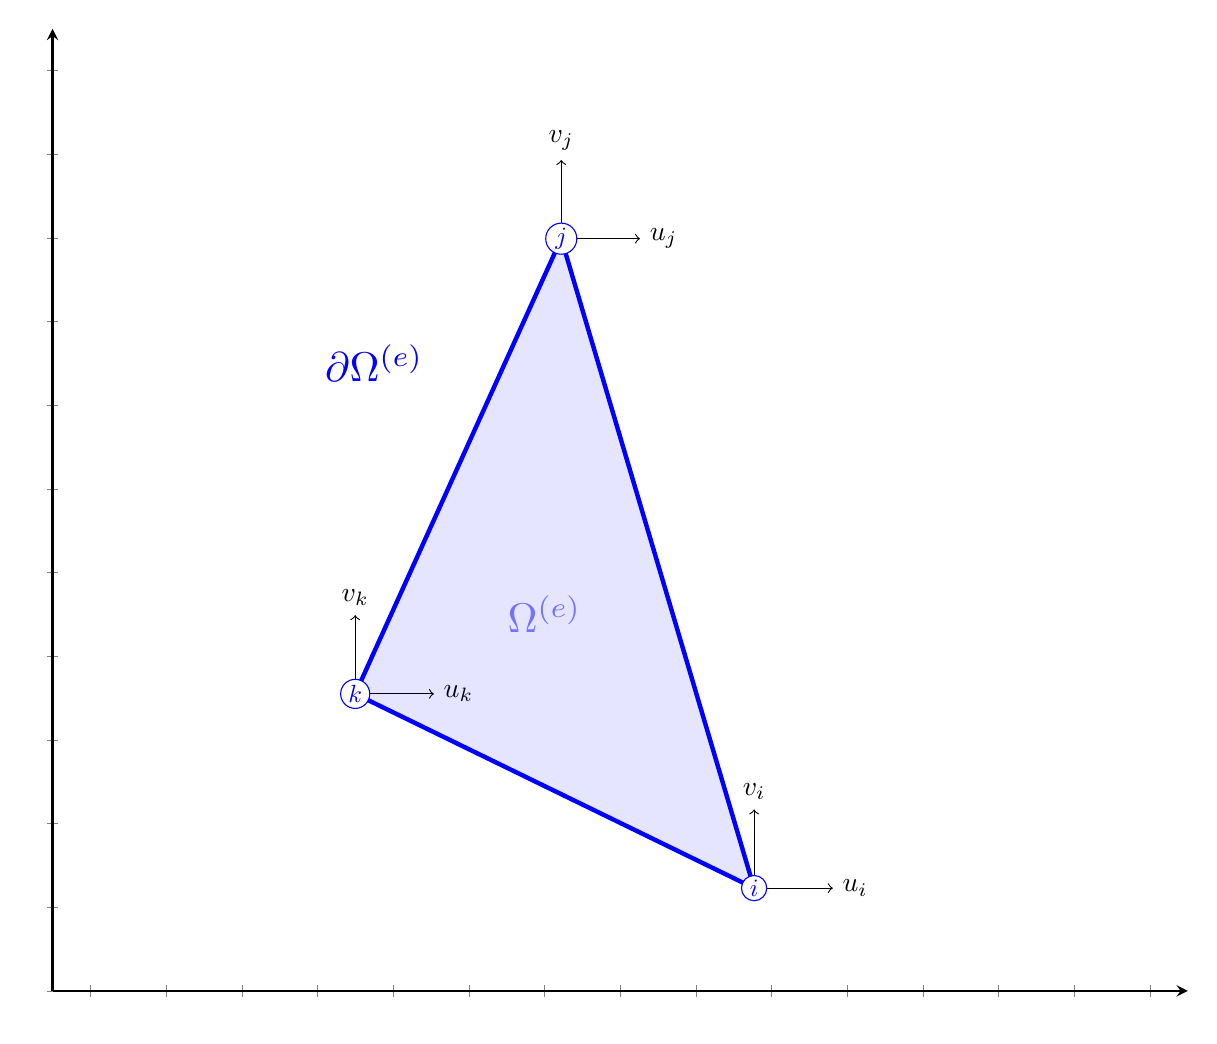
\begin{tikzpicture}
        \begin{axis}[
                xmin = -1.5, xmax = 1.5,
                ymin = -1, ymax = 1.3, 
                width = 16 cm,
                axis lines = left,
                xticklabels = {,,},
                yticklabels = {,,},
                axis line style = thick,
            ]
            \draw[->] (0.3537131,-0.7543531) -- ++(1 cm, 0 cm) node[right] {$u_i$};
            \draw[->] (0.3537131,-0.7543531) -- ++(0 cm, 1 cm) node[above] {$v_i$};
            
            \draw[->] (-0.1558111,0.798229)  -- ++(1 cm, 0 cm) node[right] {$u_j$};
            \draw[->] (-0.1558111,0.798229)  -- ++(0 cm, 1 cm) node[above] {$v_j$};

            \draw[->] (-0.7003684,-0.2899937) -- ++(1 cm, 0 cm) node[right] {$u_k$};
            \draw[->] (-0.7003684,-0.2899937) -- ++(0 cm, 1 cm) node[above] {$v_k$};

            \draw[blue, ultra thick, fill = blue, fill opacity = 0.1] 
                   (0.3537131,-0.7543531)  node[circle, draw, inner sep=1pt, fill=white, thin, scale = 0.9, fill opacity = 1] {$i$} 
                -- (-0.1558111,0.798229)   node[circle, draw, inner sep=1pt, fill=white, thin, scale = 0.9, fill opacity = 1] {$j$} 
                -- (-0.7003684,-0.2899937) node[circle, draw, inner sep=1pt, fill=white, thin, scale = 0.9, fill opacity = 1] {$k$} 
                -- cycle;
            \draw (-0.2,-0.1) node[scale = 1.5, opacity = 0.5, blue] {$\Omega^{(e)}$};
            \draw (-0.65,0.5) node[scale = 1.5, opacity = 1, blue] {$\partial\Omega^{(e)}$};
        \end{axis}
    \end{tikzpicture}
    \label{fig:CST}
	\fonte{\me{2022}}
\end{figure}

\begin{figure}
	\centering
    \caption{Um triângulo de deformações constantes sob carregamentos (CST) sob carregamentos uniformes.}
    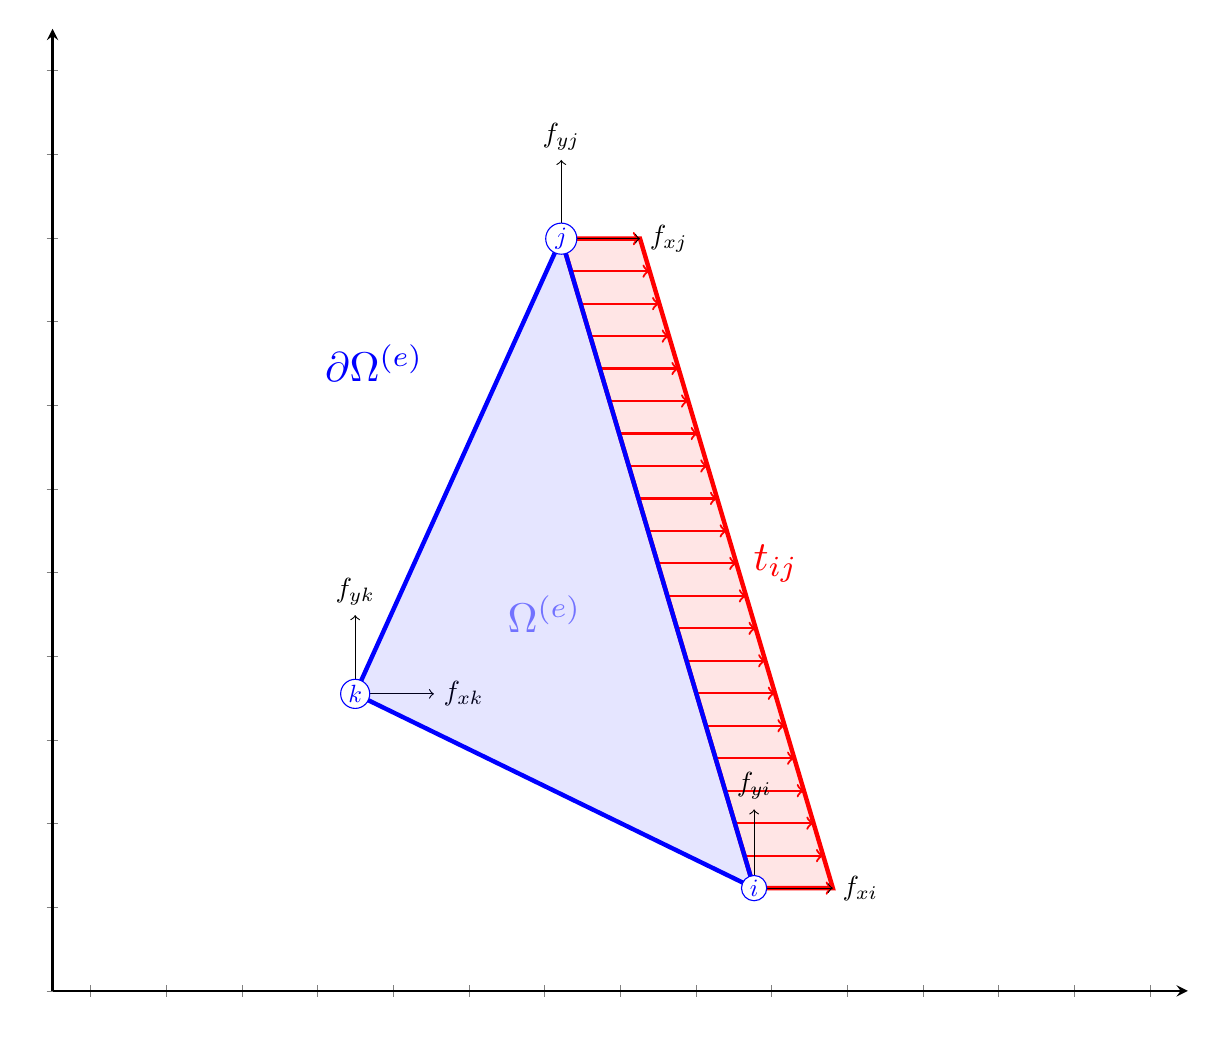
\begin{tikzpicture}
        \usetikzlibrary{calc}
        \begin{axis}[
                xmin = -1.5, xmax = 1.5,
                ymin = -1, ymax = 1.3, 
                width = 16 cm,
                axis lines = left,
                xticklabels = {,,},
                yticklabels = {,,},
                axis line style = thick,
            ]

            \coordinate  (i) at (0.3537131,-0.7543531);
            \coordinate  (j) at (-0.1558111,0.798229);
            \coordinate  (k) at (-0.7003684,-0.2899937);
            \coordinate  (ji) at ($(i)-(j)$);

            \draw[red, ultra thick, fill=red, fill opacity = 0.1]
            (j) --++ (1 cm, 0 cm) -- ($(i) + (1cm,0cm)$) -- (i) -- cycle;

            \draw[->, red, thick] (j) ++ ($ 0.0*(i)-0.0*(j)$) --++ (1cm, 0cm);
            \draw[->, red, thick] (j) ++ ($ 0.05*(i)-0.05*(j)$) --++ (1cm, 0cm);
            \draw[->, red, thick] (j) ++ ($ 0.1*(i)-0.1*(j)$) --++ (1cm, 0cm);
            \draw[->, red, thick] (j) ++ ($ 0.15*(i)-0.15*(j)$) --++ (1cm, 0cm);
            \draw[->, red, thick] (j) ++ ($ 0.2*(i)-0.2*(j)$) --++ (1cm, 0cm);
            \draw[->, red, thick] (j) ++ ($ 0.25*(i)-0.25*(j)$) --++ (1cm, 0cm);
            \draw[->, red, thick] (j) ++ ($ 0.3*(i)-0.3*(j)$) --++ (1cm, 0cm);
            \draw[->, red, thick] (j) ++ ($ 0.35*(i)-0.35*(j)$) --++ (1cm, 0cm);
            \draw[->, red, thick] (j) ++ ($ 0.4*(i)-0.4*(j)$) --++ (1cm, 0cm);
            \draw[->, red, thick] (j) ++ ($ 0.45*(i)-0.45*(j)$) --++ (1cm, 0cm);
            \draw[->, red, thick] (j) ++ ($ 0.5*(i)-0.5*(j)$) --++ (1cm, 0cm);
            \draw[->, red, thick] (j) ++ ($ 0.55*(i)-0.55*(j)$) --++ (1cm, 0cm);
            \draw[->, red, thick] (j) ++ ($ 0.6*(i)-0.6*(j)$) --++ (1cm, 0cm);
            \draw[->, red, thick] (j) ++ ($ 0.65*(i)-0.65*(j)$) --++ (1cm, 0cm);
            \draw[->, red, thick] (j) ++ ($ 0.7*(i)-0.7*(j)$) --++ (1cm, 0cm);
            \draw[->, red, thick] (j) ++ ($ 0.75*(i)-0.75*(j)$) --++ (1cm, 0cm);
            \draw[->, red, thick] (j) ++ ($ 0.8*(i)-0.8*(j)$) --++ (1cm, 0cm);
            \draw[->, red, thick] (j) ++ ($ 0.85*(i)-0.85*(j)$) --++ (1cm, 0cm);
            \draw[->, red, thick] (j) ++ ($ 0.9*(i)-0.9*(j)$) --++ (1cm, 0cm);
            \draw[->, red, thick] (j) ++ ($ 0.95*(i)-0.95*(j)$) --++ (1cm, 0cm);
            \draw[->, red, thick] (j) ++ ($ 1.0*(i)-1.0*(j)$) --++ (1cm, 0cm);

            \draw[->] (i) -- ++(1 cm, 0 cm) node[right] {$f_{xi}$};
            \draw[->] (i) -- ++(0 cm, 1 cm) node[above] {$f_{yi}$};
            
            \draw[->] (-0.1558111,0.798229)  -- ++(1 cm, 0 cm) node[right] {$f_{xj}$};
            \draw[->] (-0.1558111,0.798229)  -- ++(0 cm, 1 cm) node[above] {$f_{yj}$};

            \draw[->] (-0.7003684,-0.2899937) -- ++(1 cm, 0 cm) node[right] {$f_{xk}$};
            \draw[->] (-0.7003684,-0.2899937) -- ++(0 cm, 1 cm) node[above] {$f_{yk}$};





            \draw[blue, ultra thick, fill = blue, fill opacity = 0.1] 
                   (i)  node[circle, draw, inner sep=1pt, fill=white, thin, scale = 0.9, fill opacity = 1] {$i$} 
                -- (j)   node[circle, draw, inner sep=1pt, fill=white, thin, scale = 0.9, fill opacity = 1] {$j$} 
                -- (k) node[circle, draw, inner sep=1pt, fill=white, thin, scale = 0.9, fill opacity = 1] {$k$} 
                -- cycle;
            \draw (-0.2,-0.1) node[scale = 1.5, opacity = 0.5, blue] {$\Omega^{(e)}$};
            \draw (-0.65,0.5) node[scale = 1.5, opacity = 1, blue] {$\partial\Omega^{(e)}$};
            \draw ($0.5*(i)+0.5*(j)$) ++ (1.5 cm, 0 cm) node[red, scale=1.5] {$\bm{t}_{ij}$};
        \end{axis}
    \end{tikzpicture}
    \label{fig:CST_carregamentos}
	\fonte{\me{2022}}
\end{figure}

\section{As Funções de Interpolação}

As funções de interpolação são funções matemáticas que aproximam o campo de interesse, neste caso o deslocamento, dentro de um elemento, por meio de uma combinação linear de funções conhecidas, definidas sobre os nós do elemento. Essas funções são definidas, e depois justapostas, de modo que o campo seja contínuo. O objetivo dessa ferramente é alterar os valores incógnitos do campo de contínuos para discretos, para que o deslocamento seja bem definido pelo seu valor sobre a posição cada nó, e que, por sobre o domínio de cada elemento, o campo seja interpolado. Esses valores discretos desconhecidos do campo nos nós, em que o campo tem "liberdade" pra variar, denominam-se \emph{graus de liberdade}. \cite{LOGAN}

O CST, por exemplo, tem seis graus de liberdade, uma vez que para cada nó, o vetor de deslocamento têm três componentes. Os problemas abordados aqui têm sempre três graus de liberdade por nó.

Define-se, então, a função de deslocamento sobre um elemento, representado pela figura \ref{fig:CST}, assim como a proposta linear de interpolação,

\begin{equation}
    \bm{\varphi}^{(e)} = \begin{Bmatrix}
        u(x,y) \\ v(x,y) 
    \end{Bmatrix}^{(e)} = \begin{Bmatrix}
        a_1 + a_2 x + a_3 y \\ b_1 + b_2 x + b_3 y 
    \end{Bmatrix}^{(e)}.
\end{equation}
Nesse sentido, bidimensional, $\bm{\varphi}$ é uma função vetorial de campo que mapeia cada ponto do sólido para seu respectivo deslocamento nos eixos do sistema $xy$ ($u$ e $v$ respectivamente).

\begin{figure}
	\centering
    \caption{Um triângulo de deformações constantes (CST).}
    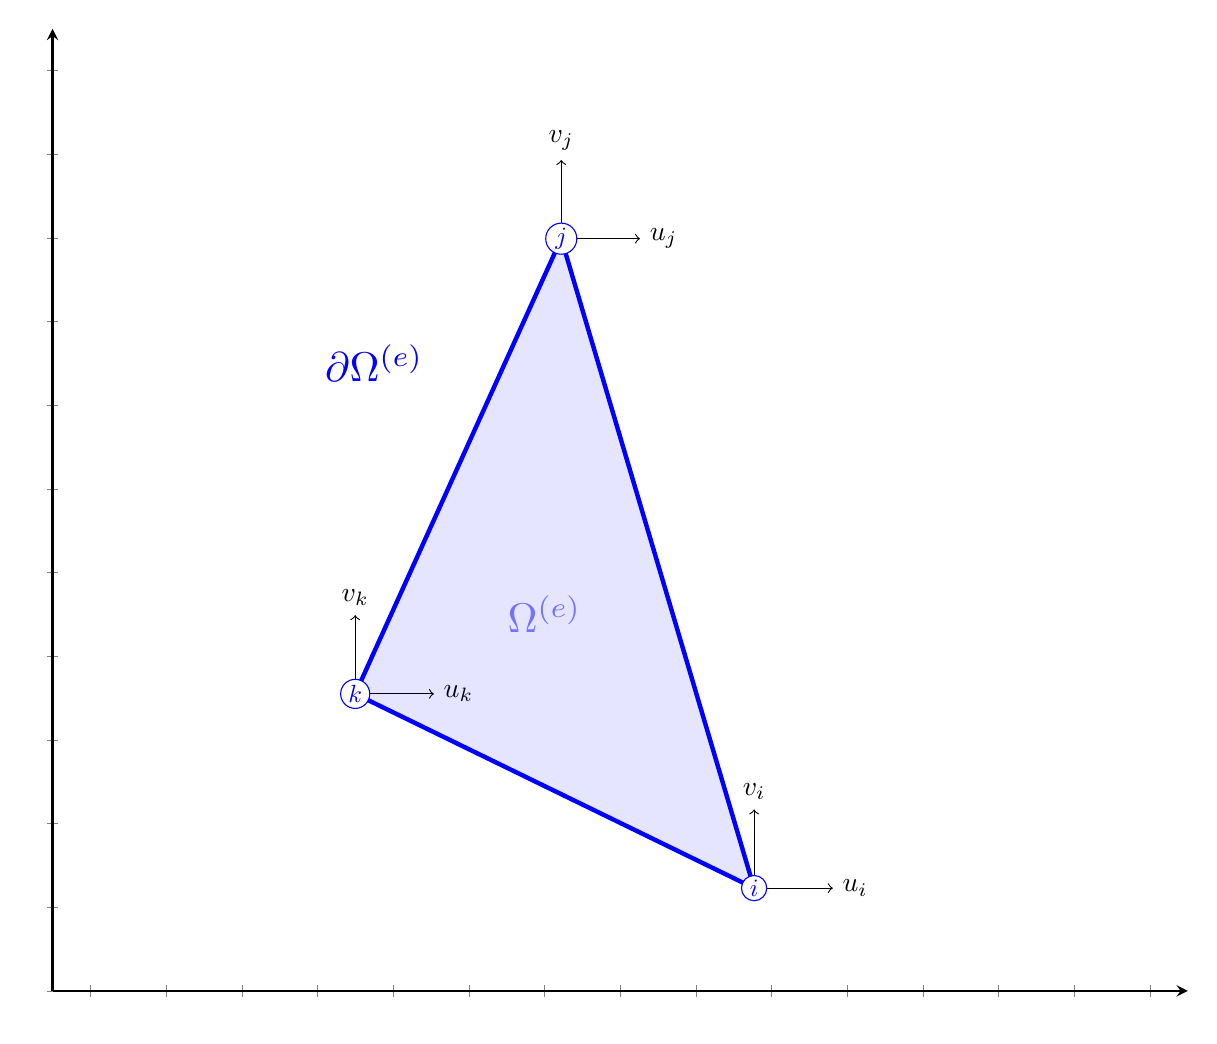
\begin{tikzpicture}
        \begin{axis}[
                xmin = -1.5, xmax = 1.5,
                ymin = -1, ymax = 1.3, 
                width = 16 cm,
                axis lines = left,
                xticklabels = {,,},
                yticklabels = {,,},
                axis line style = thick,
            ]
            \draw[->] (0.3537131,-0.7543531) -- ++(1 cm, 0 cm) node[right] {$u_i$};
            \draw[->] (0.3537131,-0.7543531) -- ++(0 cm, 1 cm) node[above] {$v_i$};
            
            \draw[->] (-0.1558111,0.798229)  -- ++(1 cm, 0 cm) node[right] {$u_j$};
            \draw[->] (-0.1558111,0.798229)  -- ++(0 cm, 1 cm) node[above] {$v_j$};

            \draw[->] (-0.7003684,-0.2899937) -- ++(1 cm, 0 cm) node[right] {$u_k$};
            \draw[->] (-0.7003684,-0.2899937) -- ++(0 cm, 1 cm) node[above] {$v_k$};

            \draw[blue, ultra thick, fill = blue, fill opacity = 0.1] 
                   (0.3537131,-0.7543531)  node[circle, draw, inner sep=1pt, fill=white, thin, scale = 0.9, fill opacity = 1] {$i$} 
                -- (-0.1558111,0.798229)   node[circle, draw, inner sep=1pt, fill=white, thin, scale = 0.9, fill opacity = 1] {$j$} 
                -- (-0.7003684,-0.2899937) node[circle, draw, inner sep=1pt, fill=white, thin, scale = 0.9, fill opacity = 1] {$k$} 
                -- cycle;
            \draw (-0.2,-0.1) node[scale = 1.5, opacity = 0.5, blue] {$\Omega^{(e)}$};
            \draw (-0.65,0.5) node[scale = 1.5, opacity = 1, blue] {$\partial\Omega^{(e)}$};
        \end{axis}
    \end{tikzpicture}
    \label{fig:CST}
	\fonte{\me{2022}}
\end{figure}

Para determinar as constantes $a$ e $b$, e termos dos deslocamentos nodais basta aplicar a condição de que em cada nó a função deve assumir o valor do deslocamento respectivo. Isto é, analisando somente a componente $x$, ou seja, $u(x,y)$, temos que

\begin{align}
    u(x_i, y_i) &= u_i = a_1 + a_2 x_i + a_3 y_i, \\
    u(x_h, y_i) &= u_j = a_1 + a_2 x_j + a_3 y_j, \\
    u(x_i, y_i) &= u_k = a_1 + a_2 x_k + a_3 y_k,
\end{align}
em que $u_i$ é o valor do deslocamento nodais $i$, assim como $x_i$ e $y_i$ é sua posição sobre o domínio $\Omega$.
 
Reescrevendo esse sistema na forma matricial, temos que

\begin{equation}
    \begin{bmatrix}
        1 & x_i & y_i \\
        1 & x_j & y_j \\
        1 & x_k & y_k \\
    \end{bmatrix}
    \begin{bmatrix}
        a_1 \\ a_2 \\ a_3
    \end{bmatrix}
    = \begin{Bmatrix}
        u_i \\ u_j \\ u_k
    \end{Bmatrix} \implies
    \begin{Bmatrix}
        a_1 \\ a_2 \\ a_3
    \end{Bmatrix} =
    \frac{1}{2A}
    \begin{bmatrix}
        \alpha_i & \alpha_j & \alpha_k \\
        \beta_i & \beta_j & \beta_k \\
        \gamma_i & \gamma_j & \gamma_k \\
    \end{bmatrix}
    \begin{Bmatrix}
        u_i \\ u_j \\ u_k
    \end{Bmatrix},
    \label{eq:matriz_x}
\end{equation}

sendo que\footnote{É fácil demonstrar que esse sistema sempre é possível e determinado apenas observando o fato de que as posições dos nós são distintas e não colineares, a final, os elementos são triangulares.}

\begin{equation}
    \frac{1}{2A}
    \begin{bmatrix}
        \alpha_i & \alpha_j & \alpha_k \\
        \beta_i & \beta_j & \beta_k \\
        \gamma_i & \gamma_j & \gamma_k \\
    \end{bmatrix} = 
    \begin{bmatrix}
        1 & x_i & y_i \\
        1 & x_j & y_j \\
        1 & x_k & y_k \\
    \end{bmatrix}^{-1} = \bm{X}^{-1},
\end{equation}
em que $A$ é área do elemento triangular. \footnote{Essa forma de escrever a inversa de $\bm{X}$ é interessante pois simplifica os termos $\alpha$, $\beta$ e $\gamma$ pelo determinante $2A$.}

Deste modo, a função de interpolação para $u(x,y)$ pode ser descrita em termos dos deslocamentos nodais na forma, utilizando o sistema \ref{eq:matriz_x},

\begin{equation}
    u(x,y) = \begin{bmatrix}
        1 & x & y
    \end{bmatrix} 
    \begin{Bmatrix}
        a_1 \\ a_2 \\ a_3
    \end{Bmatrix} = \begin{bmatrix}
        1 & x & y
    \end{bmatrix}  \frac{1}{2A}
    \begin{bmatrix}
        \alpha_i & \alpha_j & \alpha_k \\
        \beta_i & \beta_j & \beta_k \\
        \gamma_i & \gamma_j & \gamma_k \\
    \end{bmatrix}
    \begin{Bmatrix}
        u_i \\ u_j \\ u_k
    \end{Bmatrix}.
\end{equation}
Expandido essas expressões, multiplicando as matrizes e rearranjado os termos, temos que

\begin{equation}
    u(x,y) = \frac{1}{2A} \left[ \alpha_i + \beta_i x + \gamma_i y \right] u_i + \frac{1}{2A} \left[ \alpha_j + \beta_j x + \gamma_j y \right] u_j + \frac{1}{2A} \left[ \alpha_k + \beta_k x + \gamma_k y \right] u_k.
    \label{eq:funcao_u}
\end{equation}

É possível, também, definir a função de interpolação para a componente $v(x,y)$, de modo análogo, obtendo, apenas substituindo a função $u$ por $v$ nas equações anteriores, que as mesmas relações de interpolações são válidas também para a outra componente de $\bm{\varphi}$. Então, 

\begin{equation}
    v(x,y) = \frac{1}{2A} \left[ \alpha_i + \beta_i x + \gamma_i y \right] v_i + \frac{1}{2A} \left[ \alpha_j + \beta_j x + \gamma_j y \right] v_j + \frac{1}{2A} \left[ \alpha_k + \beta_k x + \gamma_k y \right] v_k.
    \label{eq:funcao_v}
\end{equation}

Para simplificar a notação das equações \ref{eq:funcao_u} e \ref{eq:funcao_v}, define-se funções $N$ da forma

\begin{align}
    N_i &= \frac{1}{2A} \left[ \alpha_i + \beta_i x + \gamma_i y \right], \\
    N_j &= \frac{1}{2A} \left[ \alpha_j + \beta_j x + \gamma_j y \right], \\
    N_k &= \frac{1}{2A} \left[ \alpha_k + \beta_k x + \gamma_k y \right].
\end{align}

Por fim, $\bm{\varphi}$ pode ser reescrito na forma matricial, em termos dessas funções $N$ e dos deslocamentos nodais e $u$ e $v$, como

\begin{equation}
    \bm{\varphi}^{(e)} = \begin{Bmatrix}
        u(x,y) \\ v(x,y)
    \end{Bmatrix}^{(e)} = \begin{bmatrix}
        N_i & 0 & N_j & 0 & N_k & 0 \\
        0 & N_i & 0 & N_j & 0 & N_k
    \end{bmatrix} \begin{Bmatrix}
        u_i \\ v_i \\ u_j \\ v_j \\ u_k \\ v_k
    \end{Bmatrix} = \bm{N} \bm{U}^{(e)},
\end{equation}
em que $\bm{N}$ é a matrix de funções de interpolação, e $\bm{U}^{(e)}$ é o vetor de deslocamentos nodais do elemento.


\section{As Relações de Tensão-Deformação-Deslocamento}

No caso bidimensional, o vetor de deformação, na notação de Voigt, é dado por, conforme definido no capítulo anterior,

\begin{equation}
    \{\epsilon\} = \begin{Bmatrix}
        \epsilon_{xx} \\ \epsilon_{yy} \\ \gamma_{xy}
    \end{Bmatrix} =
    \begin{Bmatrix}
        \frac{\partial u}{\partial x} \\ \frac{\partial v}{\partial y} \\ \frac{\partial u}{\partial y} + \frac{\partial v}{\partial x}
    \end{Bmatrix}
\end{equation}

Aplicando nessas derivadas parciais as funções de interpolação de $\bm{\varphi}$, das equações \ref{eq:funcao_u} e \ref{eq:funcao_v}, temos que, conforme \citeshort{LOGAN},

\begin{align}
    \frac{\partial u}{\partial x} &= \frac{1}{2A} \left[ \beta_i u_i + \beta_j u_j + \beta_k u_k\right],  \\
    \frac{\partial v}{\partial y} &= \frac{1}{2A} \left[ \gamma_i v_i + \gamma_j v_j + \gamma_k v_k\right],  \\
    \frac{\partial u}{\partial y} + \frac{\partial v}{\partial x} &= \frac{1}{2A} \left[ \gamma_i u_i + \gamma_j u_j + \gamma_k u_k + \beta_i v_i + \beta_j v_j + \beta_k v_k \right].
\end{align}

Utilizando essas equações, é possível reescrever o vetor de deformação $\{\epsilon\}$ em termos dos coeficientes $\beta$ e $\gamma$, como também do vetor de deslocamentos nodais do elemento $\{U\}^{(e)}$, na forma

\begin{equation}
    \{\epsilon\} = \frac{1}{2A} \begin{bmatrix}
        \beta_i & 0 & \beta_j & 0 & \beta_k & 0 \\
        0 & \gamma_i & 0 & \gamma_j & 0 & \gamma_k \\
        \gamma_i & \beta_i & \gamma_j & \beta_j & \gamma_k & \beta_k
    \end{bmatrix} \begin{Bmatrix}
        u_i \\ v_i \\ u_j \\ v_j \\ u_k \\ v_k
    \end{Bmatrix} = \bm{B} \bm{U}^{(e)}.
    \label{eq:deformacao_deslocamento}
\end{equation}

A matrix $\bm{B}$ é uma função das coordenadas dos nós do elemento, e relaciona o vetor de deslocamentos nodais do elemento $\bm{U}^{(e)}$ com o vetor de deformações $\{\epsilon\}$, assim como é constante ao longo de todo o elemento, o que é devido pela escolha de funções lineares de interpolação. Por causa dessa propriedade, esse elemento é denominado triângulo de deformações constantes, ou CST (\emph{Constant Strain Triangle}).

Por fim, ao passo que a relação entre deformação e tensão é dada pela Lei de Hooke generalizada, na forma da matriz constitutiva $\bm{C}$ (por conveniência, a matriz constitutiva será expressa sem a notação usual $[C]$), expressar a relação entre tensão e deslocamento, ou tensão-Deformação-Deslocamento, é simplesmente uma questão de multiplicar a matriz constitutiva pela matriz $\bm{B}$, obtendo assim a relação

\begin{equation}
    \{\sigma\} = \bm{C} \bm{B} \bm{U}^{(e)}.
    \label{eq:relacao_tensao_deslocamento}
\end{equation}


\section{A Matriz de Rigidez Local}

A matriz de rigidez local é uma matriz quadrada, simétrica, que relaciona o vetor de forças nodais $\bm{F}^{(e)}$ com o vetor de deslocamentos nodais $\bm{U}^{(e)}$, na forma
\begin{equation}
    \bm{F}^{(e)} = \bm{K}^{(e)} \bm{U}^{(e)},
\end{equation}
cuja derivação é feita aplicando a equação de governo, o equilíbrio estático nesse caso, sobre o elemento, utilizando as funções de interpolação para o campo de deslocamentos. \cite{LOGAN}

$\bm{F}^{(e)}$ é um vetor que armazena as forças aplicadas sobre os nós do elemento, analogamente a $\bm{U}^{(e)}$ que armazena os deslocamentos nodais, e tem a forma

\begin{equation}
    \bm{F}^{(e)} = \begin{Bmatrix}
        fx_i \\ fy_j \\ fx_j \\ fy_j \\ fx_k \\ fy_k
    \end{Bmatrix}.
\end{equation}

Um dos métodos para derivar essa matriz é utilizar o \emph{Princípio dos Trabalhos Virtuais}, que pode ser enunciado como:

\begin{citacao}
    Se um corpo deformável em equilíbrio é submetido a deslocamentos virtuais arbitrários (imaginários) associados a uma deformação compatível do corpo, o trabalho virtual das forças externas no corpo é igual à energia virtual de deformação das tensões internas. \cite[pág. 876, tradução livre]{LOGAN}
\end{citacao}

Nesse contexto, o trabalho virtual interno é causado por uma deformação do próprio corpo, denotada $\delta \bm{\epsilon}$, enquanto o trabalho virtual externo, por sua vez, é causado diretamente por um deslocamento virtual das forças que atuam sobre as fronteiras do corpo, denotado $\delta \bm{u}$. Em um corpo elástico, modelado pela Lei de Hooke, o trabalho virtual interno pode ser descrito em termos do deslocamento, como a energia armazenada na forma elástica, a fim de desenvolver as equações de equilíbrio estático apresentadas a seguir. \footnote{A notação $\delta$ se refere a um variacional, que representa uma variação infinitesimal sobre o todo o contínuo da função, de modo que seja nulo na região em que são aplicadas as condições de contorno. O cálculo variacional, entretanto, não é abordado diretamente nesta monografia.}


Seja um elemento triangular, como da figura \ref{fig:CST_carregamentos}, que sofre um deslocamento virtual $\delta \bm{U}^{(e)}$. De acordo com \citeshort{Zin}, o trabalho interno do elemento é dado por\footnote{Poder escrever a energia interna desta forma simples é devido à escolha de que, na notação de Voigt do tensor de deformação, foi utilizado a convenção de $\gamma = 2 \epsilon$.}

\begin{equation}
    \mathcal{U} = \int_{\Omega^{(e)}} \delta \{\epsilon\}^t \{\sigma\} dV,
\end{equation}

Utilizando as relações de tensão-deformação-deslocamento, descritas nas equações \ref{eq:deformacao_deslocamento} e \ref{eq:relacao_tensao_deslocamento}, temos que\footnote{Utilizando também a propriedade de transposição do produto de matrizes, $(\bm{A}\bm{B})^t = \bm{B}^t \bm{A}^t$.}

\begin{equation}
    \mathcal{U} = \int_{\Omega^{(e)}} (\bm{B} \delta \bm{U}^{(e)})^t \bm{C} \bm{B} \bm{U}^{(e)} dV
    \implies \mathcal{U} = \delta (\bm{U}^{(e)})^t \int_{\Omega^{(e)}} \bm{B}^t \bm{C} \bm{B} dV \bm{U}^{(e)}.
\end{equation}

\begin{figure}
	\centering
    \caption{Um triângulo de deformações constantes sob carregamentos (CST) sob carregamentos uniformes.}
    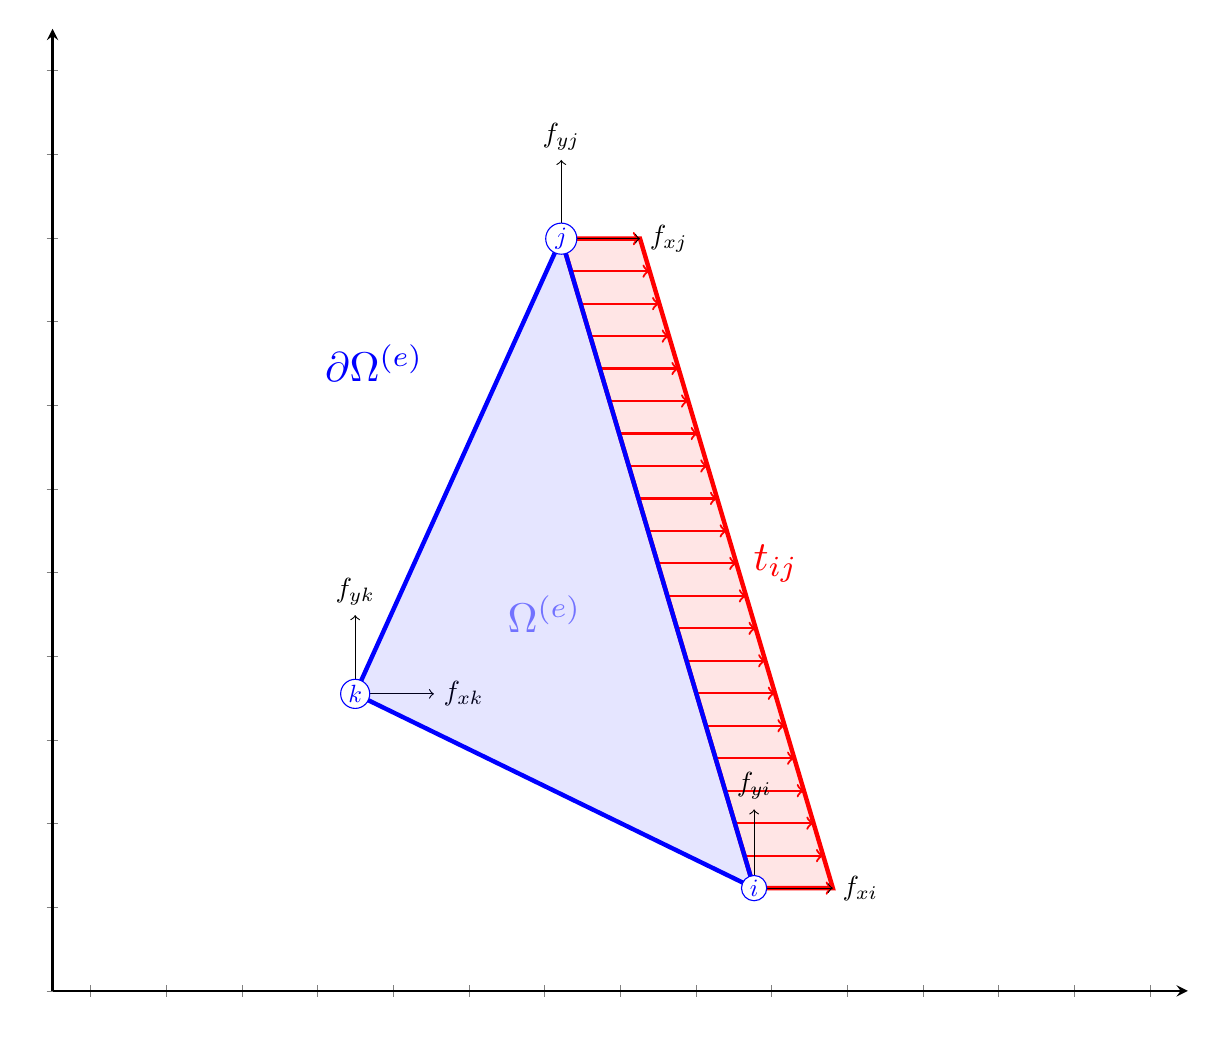
\begin{tikzpicture}
        \usetikzlibrary{calc}
        \begin{axis}[
                xmin = -1.5, xmax = 1.5,
                ymin = -1, ymax = 1.3, 
                width = 16 cm,
                axis lines = left,
                xticklabels = {,,},
                yticklabels = {,,},
                axis line style = thick,
            ]

            \coordinate  (i) at (0.3537131,-0.7543531);
            \coordinate  (j) at (-0.1558111,0.798229);
            \coordinate  (k) at (-0.7003684,-0.2899937);
            \coordinate  (ji) at ($(i)-(j)$);

            \draw[red, ultra thick, fill=red, fill opacity = 0.1]
            (j) --++ (1 cm, 0 cm) -- ($(i) + (1cm,0cm)$) -- (i) -- cycle;

            \draw[->, red, thick] (j) ++ ($ 0.0*(i)-0.0*(j)$) --++ (1cm, 0cm);
            \draw[->, red, thick] (j) ++ ($ 0.05*(i)-0.05*(j)$) --++ (1cm, 0cm);
            \draw[->, red, thick] (j) ++ ($ 0.1*(i)-0.1*(j)$) --++ (1cm, 0cm);
            \draw[->, red, thick] (j) ++ ($ 0.15*(i)-0.15*(j)$) --++ (1cm, 0cm);
            \draw[->, red, thick] (j) ++ ($ 0.2*(i)-0.2*(j)$) --++ (1cm, 0cm);
            \draw[->, red, thick] (j) ++ ($ 0.25*(i)-0.25*(j)$) --++ (1cm, 0cm);
            \draw[->, red, thick] (j) ++ ($ 0.3*(i)-0.3*(j)$) --++ (1cm, 0cm);
            \draw[->, red, thick] (j) ++ ($ 0.35*(i)-0.35*(j)$) --++ (1cm, 0cm);
            \draw[->, red, thick] (j) ++ ($ 0.4*(i)-0.4*(j)$) --++ (1cm, 0cm);
            \draw[->, red, thick] (j) ++ ($ 0.45*(i)-0.45*(j)$) --++ (1cm, 0cm);
            \draw[->, red, thick] (j) ++ ($ 0.5*(i)-0.5*(j)$) --++ (1cm, 0cm);
            \draw[->, red, thick] (j) ++ ($ 0.55*(i)-0.55*(j)$) --++ (1cm, 0cm);
            \draw[->, red, thick] (j) ++ ($ 0.6*(i)-0.6*(j)$) --++ (1cm, 0cm);
            \draw[->, red, thick] (j) ++ ($ 0.65*(i)-0.65*(j)$) --++ (1cm, 0cm);
            \draw[->, red, thick] (j) ++ ($ 0.7*(i)-0.7*(j)$) --++ (1cm, 0cm);
            \draw[->, red, thick] (j) ++ ($ 0.75*(i)-0.75*(j)$) --++ (1cm, 0cm);
            \draw[->, red, thick] (j) ++ ($ 0.8*(i)-0.8*(j)$) --++ (1cm, 0cm);
            \draw[->, red, thick] (j) ++ ($ 0.85*(i)-0.85*(j)$) --++ (1cm, 0cm);
            \draw[->, red, thick] (j) ++ ($ 0.9*(i)-0.9*(j)$) --++ (1cm, 0cm);
            \draw[->, red, thick] (j) ++ ($ 0.95*(i)-0.95*(j)$) --++ (1cm, 0cm);
            \draw[->, red, thick] (j) ++ ($ 1.0*(i)-1.0*(j)$) --++ (1cm, 0cm);

            \draw[->] (i) -- ++(1 cm, 0 cm) node[right] {$f_{xi}$};
            \draw[->] (i) -- ++(0 cm, 1 cm) node[above] {$f_{yi}$};
            
            \draw[->] (-0.1558111,0.798229)  -- ++(1 cm, 0 cm) node[right] {$f_{xj}$};
            \draw[->] (-0.1558111,0.798229)  -- ++(0 cm, 1 cm) node[above] {$f_{yj}$};

            \draw[->] (-0.7003684,-0.2899937) -- ++(1 cm, 0 cm) node[right] {$f_{xk}$};
            \draw[->] (-0.7003684,-0.2899937) -- ++(0 cm, 1 cm) node[above] {$f_{yk}$};





            \draw[blue, ultra thick, fill = blue, fill opacity = 0.1] 
                   (i)  node[circle, draw, inner sep=1pt, fill=white, thin, scale = 0.9, fill opacity = 1] {$i$} 
                -- (j)   node[circle, draw, inner sep=1pt, fill=white, thin, scale = 0.9, fill opacity = 1] {$j$} 
                -- (k) node[circle, draw, inner sep=1pt, fill=white, thin, scale = 0.9, fill opacity = 1] {$k$} 
                -- cycle;
            \draw (-0.2,-0.1) node[scale = 1.5, opacity = 0.5, blue] {$\Omega^{(e)}$};
            \draw (-0.65,0.5) node[scale = 1.5, opacity = 1, blue] {$\partial\Omega^{(e)}$};
            \draw ($0.5*(i)+0.5*(j)$) ++ (1.5 cm, 0 cm) node[red, scale=1.5] {$\bm{t}_{ij}$};
        \end{axis}
    \end{tikzpicture}
    \label{fig:CST_carregamentos}
	\fonte{\me{2022}}
\end{figure}


O trabalho desenvolvido pelas forças externas é dado, também de acordo com \citeshort{Zin}, pelo produto dos deslocamento nodais e das forças nodais, na forma

\begin{equation}
    \mathcal{W} = \delta (\bm{U}^{(e)})^t \bm{F}^{(e)}.
\end{equation}

Igualando as duas parcelas de trabalho, temos que

\begin{equation}
    \mathcal{U} =  \mathcal{W}\implies
    \delta (\bm{U}^{(e)})^t \int_{\Omega^{(e)}} \bm{B}^t \bm{C} \bm{B} dV \bm{U}^{(e)} = \delta (\bm{U}^{(e)})^t \bm{F}^{(e)}.
\end{equation}

Portanto, 

\begin{equation}
    \bm{F}^{(e)} = \int_{\Omega^{(e)}} \bm{B}^t \bm{C} \bm{B} dV \bm{U}^{(e)}.
    \label{eq:forca_equivalente}
\end{equation}

Comparando com a forma da equação \ref{eq:sistema_global}, fica evidente que a matriz de rigidez local é dada por

\begin{equation}
    \bm{K}^{(e)} = \int_{\Omega^{(e)}} \bm{B}^t \bm{C} \bm{B} dV.
\end{equation}

O elemento tratado aqui é o CST, portanto, a matriz $\bm{B}$ é constante em todo o domínio $\Omega^{(e)}$, como também é constante a matriz constitutiva $\bm{C}$. A integral, portanto, não precisa ser computada em um sistema local, pois todos os termos que a compõe são constantes. Logo, a matriz de rigidez local pode ser simplificada ainda mais, tornando-se, de acordo com \citeshort{LOGAN}

\begin{equation}
    \bm{K}^{(e)} = \bm{B}^t \bm{C} \bm{B} \int_{\Omega^{(e)}} dV = \bm{B}^t \bm{C} \bm{B} V,
    \label{eq:matriz_local}
\end{equation}
em que $V$ é o volume do elemento, definido, no caso bidimensional, por $V = A d$, em que $d$ é a espessura.

Essa matriz pode ser lida como uma lista de causa e efeito. Enquanto a linha da matriz representa onde que o efeito do deslocamento é aplicado, a força no caso, a coluna informa qual é o deslocamento, o grau de liberdade, que o causa. \cite{LOGAN}

Outra forma de derivar essa relação diretamente da equação de equilíbrio estático é por meio do método de Galerkin, em que as bases da função de interpolação são as mesmas da função de ponderação, utilizando a chamada formulação fraca da equação de governo. Esse método leva à mesma formulação mostrada acima.

Vale ressaltar que não foi preciso definir um sistema local de coordenadas para derivar essas relações, uma vez que o elemento tradado aqui, como também o tetraedro (tratado mais adiante), tem funções de interpolação simples o suficiente que um sistema orientado a cada elemento não é necessário. Elementos mais sofisticados necessitam, por uma questão de manipulação algébrica, de um sistema de referência local. Esses elementos não são tratados aqui.

\section{Matriz de Rigidez Global e Condições de Contorno}

Para cada elemento do domínio é realizado o procedimento descrito na seção anterior, de encontrar a matriz de rigidez local que descreve o equilíbrio do elemento em termos das forças externas e do campo de deslocamento sobre os nós. Para resolver o problema, encontrar os deslocamentos de todos os nós, é necessário justapor essas matrizes locais em uma matriz global, ou seja,
\begin{equation}
    \bm{K} = \sum_{e} \bm{K}^{(e)}.
\end{equation}
Nesse contexto, $\Sigma$ representa, não uma soma ordinária, mas sim a sobreposição dos efeitos de rigidez sobre os nós. \cite{LOGAN}

Em cada elemento, a matriz local de rigidez $\bm{K}^{(e)}$ define a interação de forças e deslocamentos entre os graus de liberdade dos nós. Analisando a estrutura como um todo, cada nó pode pertencer a vários elementos, pois é assim que a malha é constituída. O efeito de rigidez, então, sobre cada nó é a soma dos efeitos de todos os elementos que o contém. Isso vale para os deslocamentos nodais, como para as forças nodais. O procedimento, portanto, de montagem da matriz global de rigidez é a soma das matrizes locais de rigidez sobre as posições dos graus de liberdade respe    ctivos das matrizes locais (mapeamento local-global).

Seja um sólido $\mathcal{B}$ discretizado por uma malha composta de cinco nós, formando três elementos, conforme a figura \ref{fig:exemplo_matriz_global}, engastado na superfície inferior do elemento azulado e sujeito a uma força \textcolor{purple}{$f$} concentrada no nó $2$, como também um carregamento distribuído \textcolor{orange}{$t$} na superfície entre os nós $4$ e $5$.


\begin{figure}
	\centering
    \caption{Uma estrutura discretizada em elementos CST.}
    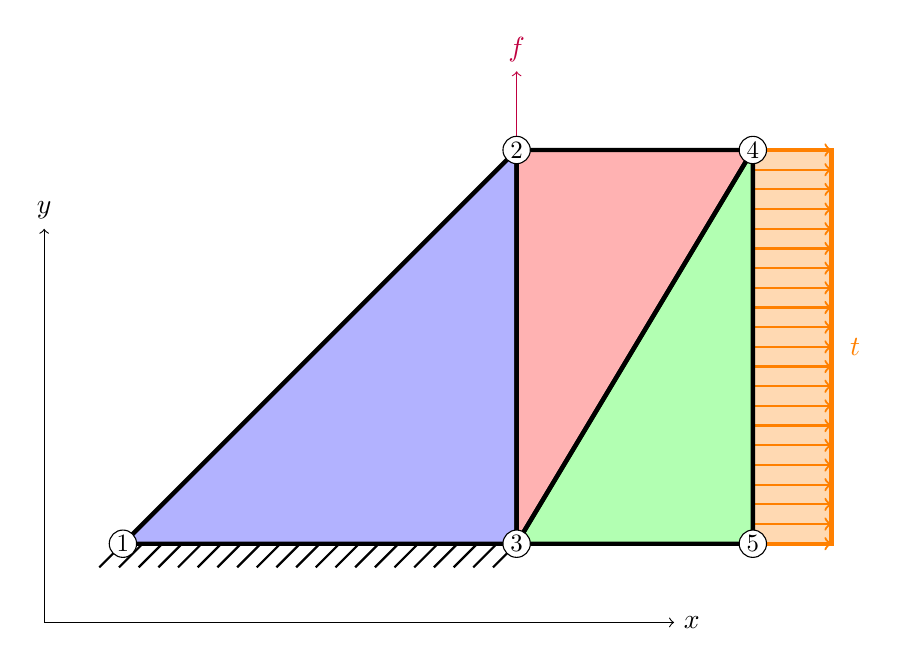
\begin{tikzpicture}
        \usetikzlibrary{calc}
        \coordinate  (1) at (0 cm,0 cm);
        \coordinate  (2) at (5 cm, 5 cm);
        \coordinate  (3) at (5 cm, 0 cm);
        \coordinate  (4) at (8 cm, 5 cm);
        \coordinate  (5) at (8 cm, 0 cm);

        \draw[orange, ultra thick, fill = orange, fill opacity = 0.3] (4) -- (5) --++ (1 cm, 0 cm) --++ (0 cm, 5 cm) -- cycle;

    
                
        \draw[->, orange, thick] (4) ++ ($ 0.0*(5)-0.0*(4)$) --++ (1cm, 0cm);
        \draw[->, orange, thick] (4) ++ ($ 0.05*(5)-0.05*(4)$) --++ (1cm, 0cm);
        \draw[->, orange, thick] (4) ++ ($ 0.1*(5)-0.1*(4)$) --++ (1cm, 0cm);
        \draw[->, orange, thick] (4) ++ ($ 0.15*(5)-0.15*(4)$) --++ (1cm, 0cm);
        \draw[->, orange, thick] (4) ++ ($ 0.2*(5)-0.2*(4)$) --++ (1cm, 0cm);
        \draw[->, orange, thick] (4) ++ ($ 0.25*(5)-0.25*(4)$) --++ (1cm, 0cm);
        \draw[->, orange, thick] (4) ++ ($ 0.3*(5)-0.3*(4)$) --++ (1cm, 0cm);
        \draw[->, orange, thick] (4) ++ ($ 0.35*(5)-0.35*(4)$) --++ (1cm, 0cm);
        \draw[->, orange, thick] (4) ++ ($ 0.4*(5)-0.4*(4)$) --++ (1cm, 0cm);
        \draw[->, orange, thick] (4) ++ ($ 0.45*(5)-0.45*(4)$) --++ (1cm, 0cm);
        \draw[->, orange, thick] (4) ++ ($ 0.5*(5)-0.5*(4)$) --++ (1cm, 0cm);
        \draw[->, orange, thick] (4) ++ ($ 0.55*(5)-0.55*(4)$) --++ (1cm, 0cm);
        \draw[->, orange, thick] (4) ++ ($ 0.6*(5)-0.6*(4)$) --++ (1cm, 0cm);
        \draw[->, orange, thick] (4) ++ ($ 0.65*(5)-0.65*(4)$) --++ (1cm, 0cm);
        \draw[->, orange, thick] (4) ++ ($ 0.7*(5)-0.7*(4)$) --++ (1cm, 0cm);
        \draw[->, orange, thick] (4) ++ ($ 0.75*(5)-0.75*(4)$) --++ (1cm, 0cm);
        \draw[->, orange, thick] (4) ++ ($ 0.8*(5)-0.8*(4)$) --++ (1cm, 0cm);
        \draw[->, orange, thick] (4) ++ ($ 0.85*(5)-0.85*(4)$) --++ (1cm, 0cm);
        \draw[->, orange, thick] (4) ++ ($ 0.9*(5)-0.9*(4)$) --++ (1cm, 0cm);
        \draw[->, orange, thick] (4) ++ ($ 0.95*(5)-0.95*(4)$) --++ (1cm, 0cm);
        \draw[->, orange, thick] (4) ++ ($ 1.0*(5)-1.0*(4)$) --++ (1cm, 0cm);
                    
        \draw[black, ultra thick, fill = blue, fill opacity = 0.3] (1) -- (2) -- (3) -- cycle;
        \draw[black, ultra thick, fill = red, fill opacity = 0.3] (2) -- (3) -- (4) -- cycle;
        \draw[black, ultra thick, fill = green, fill opacity = 0.3] (3) -- (4) -- (5) -- cycle;

        \draw[->, purple] (2) --++(0 cm, 1 cm) node[above, purple]{$f$};

        
        \draw[thick] ($0.0*(3)$) --++ (-0.3 cm, -0.3 cm);
        \draw[thick] ($0.05*(3)$) --++ (-0.3 cm, -0.3 cm);
        \draw[thick] ($0.1*(3)$) --++ (-0.3 cm, -0.3 cm);
        \draw[thick] ($0.15*(3)$) --++ (-0.3 cm, -0.3 cm);
        \draw[thick] ($0.2*(3)$) --++ (-0.3 cm, -0.3 cm);
        \draw[thick] ($0.25*(3)$) --++ (-0.3 cm, -0.3 cm);
        \draw[thick] ($0.3*(3)$) --++ (-0.3 cm, -0.3 cm);
        \draw[thick] ($0.35*(3)$) --++ (-0.3 cm, -0.3 cm);
        \draw[thick] ($0.4*(3)$) --++ (-0.3 cm, -0.3 cm);
        \draw[thick] ($0.45*(3)$) --++ (-0.3 cm, -0.3 cm);
        \draw[thick] ($0.5*(3)$) --++ (-0.3 cm, -0.3 cm);
        \draw[thick] ($0.55*(3)$) --++ (-0.3 cm, -0.3 cm);
        \draw[thick] ($0.6*(3)$) --++ (-0.3 cm, -0.3 cm);
        \draw[thick] ($0.65*(3)$) --++ (-0.3 cm, -0.3 cm);
        \draw[thick] ($0.7*(3)$) --++ (-0.3 cm, -0.3 cm);
        \draw[thick] ($0.75*(3)$) --++ (-0.3 cm, -0.3 cm);
        \draw[thick] ($0.8*(3)$) --++ (-0.3 cm, -0.3 cm);
        \draw[thick] ($0.85*(3)$) --++ (-0.3 cm, -0.3 cm);
        \draw[thick] ($0.9*(3)$) --++ (-0.3 cm, -0.3 cm);
        \draw[thick] ($0.95*(3)$) --++ (-0.3 cm, -0.3 cm);
        \draw[thick] ($1.0*(3)$) --++ (-0.3 cm, -0.3 cm);

        \draw ($0.5*(5) + 0.5*(4)$) ++ (1.3 cm, 0 cm) node[orange] {$t$};

        
        \draw (1) node[circle, draw, inner sep=1pt, fill=white, thin, scale = 0.9, fill opacity = 1] {$1$};
        \draw (2) node[circle, draw, inner sep=1pt, fill=white, thin, scale = 0.9, fill opacity = 1] {$2$};
        \draw (3) node[circle, draw, inner sep=1pt, fill=white, thin, scale = 0.9, fill opacity = 1] {$3$};
        \draw (4) node[circle, draw, inner sep=1pt, fill=white, thin, scale = 0.9, fill opacity = 1] {$4$};
        \draw (5) node[circle, draw, inner sep=1pt, fill=white, thin, scale = 0.9, fill opacity = 1] {$5$};

        \draw[->] (-1 cm, -1 cm) --++ (8 cm, 0 cm) node[right] {$x$};
        \draw[->] (-1 cm, -1 cm) --++ (0 cm, 5 cm) node[above] {$y$};
    \end{tikzpicture}
    \label{fig:exemplo_matriz_global}
    \fonte{\me{2022}}
\end{figure}

As matrizes locais de rigidez desses elementos são quadradas $6 \times 6$, pois no CST existem três graus de liberdade, dois para cada nó, referente ao deslocamento nas direções de $x$ e $y$. Os sistemas locas, então, para elemento da figura \ref{fig:exemplo_matriz_global}, têm a forma

\begin{align}
    \color{blue} \begin{bmatrix}
        k_{11} & k_{12} & k_{13} & k_{14} & k_{15} & k_{16} \\
        k_{21} & k_{22} & k_{23} & k_{24} & k_{25} & k_{26} \\
        k_{31} & k_{32} & k_{33} & k_{34} & k_{35} & k_{36} \\
        k_{41} & k_{42} & k_{43} & k_{44} & k_{45} & k_{46} \\
        k_{51} & k_{52} & k_{53} & k_{54} & k_{55} & k_{56} \\
        k_{61} & k_{62} & k_{63} & k_{64} & k_{65} & k_{66} \\
    \end{bmatrix}^{(1)}
    \color{black}
    \begin{Bmatrix}
        u_1 \\ v_1 \\ u_2 \\ v_2 \\ u_3 \\ v_3
    \end{Bmatrix}
    &=
    \begin{Bmatrix}
        f_{x1} \\ f_{y1} \\ f_{x2} \\ f_{y2} \\ f_{x3} \\ f_{y3}
    \end{Bmatrix} \iff \color{blue} \bm{K}^{(e)} \bm{U}^{(e)} = \bm{F}^{(e)}, \\
    \color{red} \begin{bmatrix}
        k_{11} & k_{12} & k_{13} & k_{14} & k_{15} & k_{16} \\
        k_{21} & k_{22} & k_{23} & k_{24} & k_{25} & k_{26} \\
        k_{31} & k_{32} & k_{33} & k_{34} & k_{35} & k_{36} \\
        k_{41} & k_{42} & k_{43} & k_{44} & k_{45} & k_{46} \\
        k_{51} & k_{52} & k_{53} & k_{54} & k_{55} & k_{56} \\
        k_{61} & k_{62} & k_{63} & k_{64} & k_{65} & k_{66} \\
    \end{bmatrix}^{(2)}
    \color{black}
    \begin{Bmatrix}
        u_2 \\ v_2 \\ u_3 \\ v_3 \\ u_4 \\ v_4
    \end{Bmatrix}
    &=
    \begin{Bmatrix}
        f_{x2} \\ f_{y2} \\ f_{x3} \\ f_{y3} \\ f_{x4} \\ f_{y4}
    \end{Bmatrix} \iff \color{red} \bm{K}^{(e)} \bm{U}^{(e)} = \bm{F}^{(e)}, \\
    \color{green} \begin{bmatrix}
        k_{11} & k_{12} & k_{13} & k_{14} & k_{15} & k_{16} \\
        k_{21} & k_{22} & k_{23} & k_{24} & k_{25} & k_{26} \\
        k_{31} & k_{32} & k_{33} & k_{34} & k_{35} & k_{36} \\
        k_{41} & k_{42} & k_{43} & k_{44} & k_{45} & k_{46} \\
        k_{51} & k_{52} & k_{53} & k_{54} & k_{55} & k_{56} \\
        k_{61} & k_{62} & k_{63} & k_{64} & k_{65} & k_{66} \\
    \end{bmatrix}^{(3)}
    \color{black}
    \begin{Bmatrix}
        u_3 \\ v_3 \\ u_5 \\ v_5 \\ u_4 \\ v_4
    \end{Bmatrix}
    &=
    \begin{Bmatrix}
        f_{x3} \\ f_{y3} \\ f_{x5} \\ f_{y5} \\ f_{x4} \\ f_{y4}
    \end{Bmatrix} \iff \color{green} \bm{K}^{(e)} \bm{U}^{(e)} = \bm{F}^{(e)}.
\end{align}

A montagem do sistema global é somar essas matrizes de rigidez sobre os graus de liberdade. Observemos que o primeiro nó só faz parte de um elemento, o \textcolor{blue}{azul}, portanto sua rigidez só tem contribuição desse elemento; o nó $3$, por sua vez, pertence aos três elementos (\textcolor{blue}{azul}, \textcolor{red}{vermelho} e \textcolor{green}{verde}), e, portanto, seu termo de rigidez tem contribuição de todos eles. Realizando esse procedimento, é possível montar a matriz global de rigidez, utilizando, para tanto, a notação dos vetores de deslocamentos nodais $\bm{U}$ e de forças nodais $\bm{F}$.

A matriz de rigidez global é quadrada $10 \times 10$, pois existem cinco nós, com dois graus de liberdade cada, e é dada por
\begin{landscape}
    \begin{equation}
            \begin{bmatrix}
                \textcolor{blue}{k_{11}} &  \textcolor{blue}{k_{12}} &  \textcolor{blue}{k_{13}}                           &  \textcolor{blue}{k_{14}}                             &  \textcolor{blue}{k_{15}}                                                       &  \textcolor{blue}{k_{16}}                                                       & 0                                                    & 0                                                    & 0                          & 0                          \\
                \textcolor{blue}{k_{21}} &  \textcolor{blue}{k_{22}} &  \textcolor{blue}{k_{23}}                           &  \textcolor{blue}{k_{24}}                             &  \textcolor{blue}{k_{25}}                                                       &  \textcolor{blue}{k_{26}}                                                       & 0                                                    & 0                                                    & 0                          & 0                          \\
                \textcolor{blue}{k_{31}} &  \textcolor{blue}{k_{32}} &  \textcolor{blue}{k_{33}} + \textcolor{red}{k_{11}} &  \textcolor{blue}{k_{34}} + \textcolor{red}{k_{12}}   &  \textcolor{blue}{k_{35}} + \textcolor{red}{k_{13}}                             &  \textcolor{blue}{k_{36}} + \textcolor{red}{k_{14}}                             &  \textcolor{red}{k_{15}}                             &  \textcolor{red}{k_{16}}                             & 0                          & 0                          \\
                \textcolor{blue}{k_{41}} &  \textcolor{blue}{k_{42}} &  \textcolor{blue}{k_{43}} + \textcolor{red}{k_{21}} &  \textcolor{blue}{k_{44}} + \textcolor{red}{k_{22}}   &  \textcolor{blue}{k_{45}} + \textcolor{red}{k_{23}}                             &  \textcolor{blue}{k_{46}} + \textcolor{red}{k_{24}}                             &  \textcolor{red}{k_{25}}                             &  \textcolor{red}{k_{26}}                             & 0                          & 0                          \\
                \textcolor{blue}{k_{51}} &  \textcolor{blue}{k_{52}} &  \textcolor{blue}{k_{53}} + \textcolor{red}{k_{31}} &  \textcolor{blue}{k_{54}} + \textcolor{red}{k_{32}}   &  \textcolor{blue}{k_{55}} + \textcolor{red}{k_{33}} + \textcolor{green}{k_{11}} &  \textcolor{blue}{k_{56}} + \textcolor{red}{k_{34}} + \textcolor{green}{k_{12}} &  \textcolor{red}{k_{35}} + \textcolor{green}{k_{13}} &  \textcolor{red}{k_{36}} + \textcolor{green}{k_{14}} &  \textcolor{green}{k_{15}} &  \textcolor{green}{k_{16}} \\
                \textcolor{blue}{k_{61}} &  \textcolor{blue}{k_{62}} &  \textcolor{blue}{k_{63}} + \textcolor{red}{k_{41}} &  \textcolor{blue}{k_{64}} + \textcolor{red}{k_{42}}   &  \textcolor{blue}{k_{65}} + \textcolor{red}{k_{43}} + \textcolor{green}{k_{21}} &  \textcolor{blue}{k_{66}} + \textcolor{red}{k_{44}} + \textcolor{green}{k_{22}} &  \textcolor{red}{k_{45}} + \textcolor{green}{k_{23}} &  \textcolor{red}{k_{46}} + \textcolor{green}{k_{24}} &  \textcolor{green}{k_{25}} &  \textcolor{green}{k_{26}} \\
                0                        & 0                         &  \textcolor{red}{k_{51}} &  \textcolor{red}{k_{52}} &  \textcolor{red}{k_{53}} + \textcolor{green}{k_{31}}  &  \textcolor{red}{k_{54}} + \textcolor{green}{k_{32}}                            &  \textcolor{red}{k_{55}} + \textcolor{green}{k_{33}}                            &  \textcolor{red}{k_{56}} + \textcolor{green}{k_{34}} &  \textcolor{green}{k_{35}}                           &  \textcolor{green}{k_{36}} & 0                          \\
                0                        & 0                         &  \textcolor{red}{k_{61}} &  \textcolor{red}{k_{62}} &  \textcolor{red}{k_{63}} + \textcolor{green}{k_{41}}  &  \textcolor{red}{k_{64}} + \textcolor{green}{k_{42}}                            &  \textcolor{red}{k_{65}} + \textcolor{green}{k_{43}}                            &  \textcolor{red}{k_{66}} + \textcolor{green}{k_{44}} &  \textcolor{green}{k_{45}}                           &  \textcolor{green}{k_{46}} & 0                          \\
                0                        & 0                         & 0                                                   & 0                                                     &  \textcolor{green}{k_{51}}                                                      &  \textcolor{green}{k_{52}}                                                      &  \textcolor{green}{k_{53}}                           &  \textcolor{green}{k_{54}}                           &  \textcolor{green}{k_{55}} &  \textcolor{green}{k_{56}} \\
                0                        & 0                         & 0                                                   & 0                                                     &  \textcolor{green}{k_{61}}                                                      &  \textcolor{green}{k_{62}}                                                      &  \textcolor{green}{k_{63}}                           &  \textcolor{green}{k_{64}}                           &  \textcolor{green}{k_{65}} &  \textcolor{green}{k_{66}} 
            \end{bmatrix}
            \begin{Bmatrix}
                0 \\ 0 \\ u_2 \\ v_2 \\ 0 \\ 0 \\ u_4 \\ v_4 \\ u_5 \\ v_5
            \end{Bmatrix} = 
            \begin{Bmatrix}
                R_{x1} \\ R_{y1} \\ 0 \\ \textcolor{purple}{f} \\ R_{x3} \\ R_{y3} \\ \frac{1}{2} \ell_{4-5} \textcolor{orange}{t} \\ 0 \\ \frac{1}{2} \ell_{4-5} \textcolor{orange}{t} \\ 0
            \end{Bmatrix}.
        \label{eq:sistema_global_montado}
    \end{equation}
\end{landscape}
Nas duas primeiras linhas do sistema, que representam as forças nodais sobre o primeiro nó, é possível notar que somente os deslocamentos do elemento azulado que impactam diretamente. Nos graus de $u_3$ e $u_v$, fica evidente que todos os elementos contribuem para as forças nodais do nó $3$, conforme descrito anteriormente.

Um outro passo nessa montagem do sistema global é a aplicação das condições de contorno. As condições de contorno, tradas aqui, podem ser dividas em dois tipos: 

\begin{enumerate}
    \item de Dirichlet, ou de primeiro tipo, e
    \item de Neumann, ou de segundo tipo.
\end{enumerate}

 As condições de Dirichlet são aquelas que definem valores da variável incógnita na fronteira do domínio. Já as de Neumann, são aquelas que definem valores de contorno sobre a derivada da variável incógnita nas fronteiras do domínio \cite{sinan}. Aqui, as condições de contorno de Dirichlet são restrições de deslocamento, enquanto as condições de Neumann são carregamentos aplicados sobre a estrutura.
 
As condições de contorno sobre os deslocamentos, então, dividem os graus de liberdade entre 

\begin{enumerate}
    \item livre;
    Quando não há informação prévia de seus valores, isto é, o campo pode variar livremente.
    \item prescritos;
    prescritos quando há informação prévia de seus valores, e portanto, não podem variar.
    \cite{LOGAN}
\end{enumerate}

Um engaste, por exemplo, gera uma condições de contorno de Dirichlet, definindo graus de liberdade prescritos, pois impõe que o deslocamento naquela região do sólido é nulo. Um deslocamento conhecido, também o faz, determinando que os graus correspondentes recebam o valor deslocado.

O vetor de forças $\bm{F}$ é nulo em regra sobre os graus de liberdade livres, pois essa entidade representa as forças externas sobre o elemento. Entretanto, como no MEF os deslocamentos são discretizados nos nós, o mesmo é feito com os carregamentos. Quando se aplicam condições de contorno de Neumann, os graus correspondentes devem receber forças nodais equivalentes, de forma que representem os carregamentos por forças externas concentradas nos nó. Pode-se encontrar as forças nodais equivalentes utilizando o mesmo método da seção anterior: o princípio dos trabalhos virtuais, fazendo com que o trabalho de carregamentos sobre a fronteira de um elemento $\partial \Omega^{(e)}$, causado por um deslocamento virtual $\delta \bm{U}^{(e)}$, seja igual ao trabalho da forças nodais equivalentes. Em termos matemáticos, de acordo com \citeshort{Zin},
\begin{equation}
    \delta (\bm{U}^{(e)})^t \bm{F}^{(e)} = \int_{\partial \Omega^{(e)}} (\bm{N}\bm{U}^{(e)})^t \bm{t} d \ell,
\end{equation}
em que $\bm{t}$ é o vetor do carregamento sobre a fronteira do elemento, na forma
\begin{equation}
    \bm{t} = \begin{Bmatrix}
        t_x(x,y) \\ t_y(x,y),
    \end{Bmatrix}.
\end{equation}
e $d\ell$ é o infinitesimal de área da fronteira do elemento.

Aqui os carregamentos são constantes sobre as fronteiras dos elementos, isto é, são carregamentos distribuídos e uniformes. Deste modo, a equação anterior pode ser simplificada para

\begin{equation}
    \delta (\bm{U}^{(e)})^t \bm{F}^{(e)} = \delta \bm{U}^{(e)} \int_{\partial \Omega^{(e)}} \bm{N}^t d\ell \bm{t}. 
\end{equation}
Portanto, as forças nodais equivalentes, devidas a carregamentos uniformes sobre a fronteira do elemento, é dada por
\begin{equation}
    \bm{F}^{(e)} = \int_{\partial \Omega^{(e)}} \bm{N}^t dl \bm{t}.
\end{equation}

No elemento CST, pela simplicidade das funções de interpolação, é possível realizar essa integração analiticamente. A solução mostra que o carregamento uniforme sobre a fronteira do elemento é equivalente à distribuição dessa carga duas forças nodais iguais, agindo nas extremidades da face em que atua o carregamento, ou seja, de acordo com \cite{Onate},
\begin{equation}
    \bm{F}^{(e)}_{\bm{t}} = \frac{1}{2} l^{(e)} \bm{t}
\end{equation}
em que $\bm{F}^{(e)}_{\bm{t}}$ são as forças equivalentes que compreendem a fronteira em que o carregamento $\bm{t}$ é aplicado, $l^{(e)}$ é o comprimento da fronteira do elemento, e $d$ é a espessura do elemento.

Na equação \ref{eq:sistema_global_montado}, em que foi montado o sistema global, já foram aplicada essas condições de contorno. Pode-se notar que os deslocamentos vinculados à fronteira compostas pelos nós $1$ e $3$ são nulos, pois alí se faz um engaste. A força roxeada \textcolor{purple}{$f$}, agindo sobre o nó $2$, faz-se presente diretamente no vetor de forças nodais, pois já é uma força concentrada em um nó. O carregamento alaranjado \textcolor{orange}{$t$}, por sua vez, foi decomposto em duas parcelas, para os nós $5$ e $4$, seguindo a expressão da equação anterior. 

Vale ressaltar que nos graus de liberdade prescritos as forças nodais desconhecidas são as reações das estruturas, isto é, as forças de reação que as restrições fazem sobre o corpo que se mantenha em equilíbrio. Por conta disso, na equação \ref{eq:sistema_global_montado}, as forças sobre os graus prescritos foram denominadas $R$, de reação.

\subsection{Solução direta do sistema global}

Com a determinação da matriz de rigidez global, as condições de contorno devidamente expressas em graus prescritos e livres (sejam deslocamento ou carregamentos), é possível reescrever o sistema geral da equação \ref{eq:sistema_global} na forma, de acordo com \citeshort{rao},

\begin{equation}
    \begin{bmatrix}
        \bm{K}_{LL} & \bm{K}_{LP} \\
        \bm{K}_{PL} & \bm{K}_{PP}
    \end{bmatrix} 
    \begin{Bmatrix}
        \bm{U}_L \\ \bm{U}_P
    \end{Bmatrix}
    = \begin{Bmatrix}
        \bm{F}_L \\ \bm{F}_P
    \end{Bmatrix},
    \label{eq:sistema_global_dividido}
\end{equation}
Nessa expressão, os graus de liberdade subdividem os vetores $\bm{U}$ e $\bm{F}$ em dois cada um, em prescritos ($\bm{U}_P$ e $\bm{F}_P$), e livres ($\bm{U}_L$ e $\bm{F}_L$). A matriz de rigidez, então, é subdividida em quatro, que relacionam os graus de liberdade prescritos e livros dos deslocamentos e das forças nodais, respectivamente.

Portanto, o sistema global pode ser reescrito mais uma vez em termos dessas submatrizes, como

\begin{align}
    \bm{K}_{LL} \bm{U}_L + \bm{K}_{LP} \bm{U}_P &= \bm{F}_L \\
    \bm{K}_{PL} \bm{U}_L + \bm{K}_{PP} \bm{U}_P &= \bm{F}_P.
\end{align}

Os valores conhecidos desse sistema são os deslocamentos sobre os graus prescritos $\bm{U}_P$, e as forças externas sobre o graus livres $\bm{F}_L$, a final, são as próprias condições de contorno definidas matematicamente pelo MEF. Logo, como o objetivo de resolver o sistema é encontrar os deslocamentos nodais, é possível isolar $\bm{U}_L$ na primeira equação, ou seja,

\begin{align}
    \bm{U}_L &= \bm{K}_{LL}^{-1} (\bm{F}_L - \bm{K}_{LP} \bm{U}_P), \\
    \bm{F}_P &= \bm{K}_{PL} \bm{U}_L + \bm{K}_{PP} \bm{U}_P.
\end{align}
a matriz $\bm{K}_{LL}$ é quadrada, simétrica e sempre possui inversa quando o problema está estaticamente determinado. \cite{rao}

Aplicando essas expressões à equação \ref{eq:sistema_global_montado}, referente ao exemplo da figura \ref{fig:exemplo_matriz_global}, temos que
\begin{landscape}
    \begin{align*}
        \begin{bmatrix}
            \textcolor{blue}{k_{33}} + \textcolor{red}{k_{11}} &  \textcolor{blue}{k_{34}} + \textcolor{red}{k_s{12}} &  \textcolor{red}{k_{15}} &  \textcolor{red}{k_{16}} & 0 & 0 & \\ 
            \textcolor{blue}{k_{43}} + \textcolor{red}{k_{21}} &  \textcolor{blue}{k_{44}} + \textcolor{red}{k_{22}} &  \textcolor{red}{k_{25}} &  \textcolor{red}{k_{26}} & 0 & 0 & \\ 
            \textcolor{red}{k_{51}} &  \textcolor{red}{k_{52}} &  \textcolor{red}{k_{55}} + \textcolor{green}{k_{33}} &  \textcolor{red}{k_{56}} + \textcolor{green}{k_{34}} &  \textcolor{green}{k_{35}} &  \textcolor{green}{k_{36}} & \\ 
            \textcolor{red}{k_{61}} &  \textcolor{red}{k_{62}} &  \textcolor{red}{k_{65}} + \textcolor{green}{k_{43}} &  \textcolor{red}{k_{66}} + \textcolor{green}{k_{44}} &  \textcolor{green}{k_{45}} &  \textcolor{green}{k_{46}} & \\ 
        0 & 0 &  \textcolor{green}{k_{53}} &  \textcolor{green}{k_{54}} &  \textcolor{green}{k_{55}} &  \textcolor{green}{k_{56}} & \\ 
        0 & 0 &  \textcolor{green}{k_{63}} &  \textcolor{green}{k_{64}} &  \textcolor{green}{k_{65}} &  \textcolor{green}{k_{66}} & \\ 
        \end{bmatrix}
        \begin{Bmatrix}
            u_2 \\ v_2 \\ u_4 \\ v_4 \\ u_5 \\ v_5
        \end{Bmatrix} +
        \begin{bmatrix}
            \textcolor{blue}{k_{31}} &  \textcolor{blue}{k_{32}} &  \textcolor{blue}{k_{35}} + \textcolor{red}{k_{13}} &  \textcolor{blue}{k_{36}} + \textcolor{red}{k_{14}} & \\ 
            \textcolor{blue}{k_{41}} &  \textcolor{blue}{k_{42}} &  \textcolor{blue}{k_{45}} + \textcolor{red}{k_{23}} &  \textcolor{blue}{k_{46}} + \textcolor{red}{k_{24}} & \\ 
        0 & 0 &  \textcolor{red}{k_{53}} + \textcolor{green}{k_{31}} &  \textcolor{red}{k_{54}} + \textcolor{green}{k_{32}} & \\ 
        0 & 0 &  \textcolor{red}{k_{63}} + \textcolor{green}{k_{41}} &  \textcolor{red}{k_{64}} + \textcolor{green}{k_{42}} & \\ 
        0 & 0 &  \textcolor{green}{k_{51}} &  \textcolor{green}{k_{52}} & \\ 
        0 & 0 &  \textcolor{green}{k_{61}} &  \textcolor{green}{k_{62}} & \\ 
        \end{bmatrix}
        \begin{Bmatrix}
            0 \\ 0 \\ 0 \\ 0
        \end{Bmatrix} &=
        \begin{Bmatrix}
            0 \\ \textcolor{purple}{f} \\ \frac{1}{2} \ell_{4-5} \textcolor{orange}{t} \\ 0 \\ \frac{1}{2} \ell_{4-5} \textcolor{orange}{t} \\ 0
        \end{Bmatrix} \\
        \begin{bmatrix}
            \textcolor{blue}{k_{13}} &  \textcolor{blue}{k_{14}} & 0 & 0 & 0 & 0 & \\ 
            \textcolor{blue}{k_{23}} &  \textcolor{blue}{k_{24}} & 0 & 0 & 0 & 0 & \\ 
            \textcolor{blue}{k_{53}} + \textcolor{red}{k_{31}} &  \textcolor{blue}{k_{54}} + \textcolor{red}{k_{32}} &  \textcolor{red}{k_{35}} + \textcolor{green}{k_{13}} &  \textcolor{red}{k_{36}} + \textcolor{green}{k_{14}} &  \textcolor{green}{k_{15}} &  \textcolor{green}{k_{16}} & \\ 
            \textcolor{blue}{k_{63}} + \textcolor{red}{k_{41}} &  \textcolor{blue}{k_{64}} + \textcolor{red}{k_{42}} &  \textcolor{red}{k_{45}} + \textcolor{green}{k_{23}} &  \textcolor{red}{k_{46}} + \textcolor{green}{k_{24}} &  \textcolor{green}{k_{25}} &  \textcolor{green}{k_{26}} & \\ 
        \end{bmatrix} 
        \begin{Bmatrix}
            u_2 \\ v_2 \\ u_4 \\ v_4 \\ u_5 \\ v_5
        \end{Bmatrix} + 
        \begin{bmatrix}
            \textcolor{blue}{k_{11}} &  \textcolor{blue}{k_{12}} &  \textcolor{blue}{k_{15}} &  \textcolor{blue}{k_{16}} & \\ 
            \textcolor{blue}{k_{21}} &  \textcolor{blue}{k_{22}} &  \textcolor{blue}{k_{25}} &  \textcolor{blue}{k_{26}} & \\ 
            \textcolor{blue}{k_{51}} &  \textcolor{blue}{k_{52}} &  \textcolor{blue}{k_{55}} + \textcolor{red}{k_{33}} + \textcolor{green}{k_{11}} &  \textcolor{blue}{k_{56}} + \textcolor{red}{k_{34}} + \textcolor{green}{k_{12}} & \\ 
            \textcolor{blue}{k_{61}} &  \textcolor{blue}{k_{62}} &  \textcolor{blue}{k_{65}} + \textcolor{red}{k_{43}} + \textcolor{green}{k_{21}} &  \textcolor{blue}{k_{66}} + \textcolor{red}{k_{44}} + \textcolor{green}{k_{22}} & \\ 
        \end{bmatrix}
        \begin{Bmatrix}
            0 \\ 0 \\ 0 \\ 0
        \end{Bmatrix}  &=
        \begin{Bmatrix}
            R_{x1} \\ R_{y1} \\ R_{x3} \\ R_{y3}
        \end{Bmatrix}
    \end{align*}
\end{landscape}

\section{Expressões para o Tetraedro Linear}

As mesmas relações gerais da seção anterior podem ser utilizadas para derivar as expressões para o elemento tetraédrico linear (figura \ref{fig:tetraedro}). A grande diferença é a passagem de uma modelagem bidimensional para uma tridimensional, o que implica em um aumento do número de graus de liberdade, e o abandono de EPT e EPD, como também a introdução de um nova condição de contorno sobre superfícies propriamente. De modo similar ao CST, o tetraedro é definido por três nós, nomeados $i$, $j$, $k$ e $m$, sobre os quais tanto o deslocamento é discretizado.

\begin{figure} 
    \centering
    \caption{Elemento tetraédrico}
    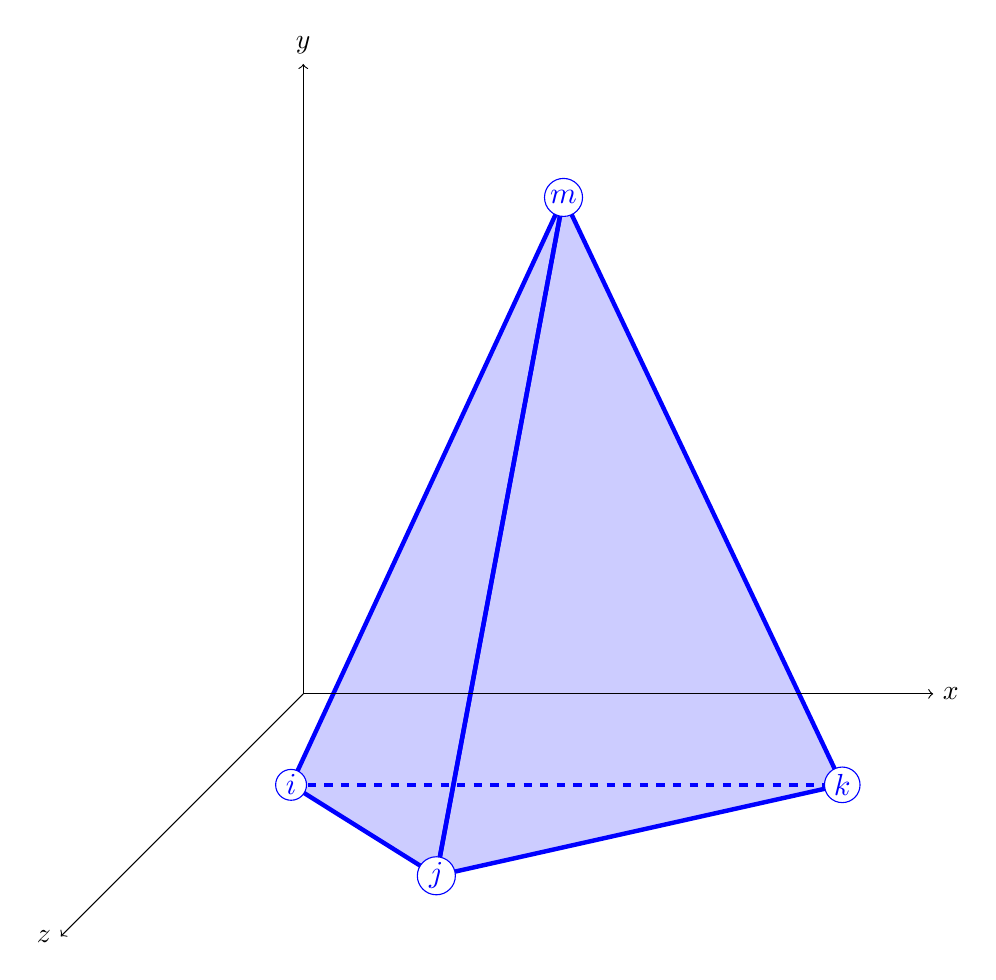
\begin{tikzpicture}
            \coordinate (i) at (1,0,3);
            \coordinate (j) at (4,0,6);
            \coordinate (k) at (8,0,3);
            \coordinate (m) at (6,9,7);
            
            \draw[blue, ultra thick, fill=blue, fill opacity = 0.2] 
                (j) 
                -- (m) -- (k)  
                -- cycle;
            \draw[blue, ultra thick, fill=blue, fill opacity = 0.2] 
            (i) -- (m) -- (j) -- cycle;
            \draw [->] (0,0,0) -- (8,0,0) node[anchor = west] {$x$};
            \draw [->] (0,0,0) -- (0,8,0) node[anchor = south] {$y$};
            \draw [->] (0,0,0) -- (0,0,8) node[anchor = east] {$z$};
            \draw[dashed, blue, ultra thick] (i) -- (k);
            \draw (i) node[blue, circle, draw, inner sep=1pt, fill=white, thin, scale = 1.1, fill opacity = 1] {$i$};
            \draw (j) node[blue, circle, draw, inner sep=1pt, fill=white, thin, scale = 1.1, fill opacity = 1] {$j$};
            \draw (k) node[blue, circle, draw, inner sep=1pt, fill=white, thin, scale = 1.1, fill opacity = 1] {$k$};
            \draw (m) node[blue, circle, draw, inner sep=1pt, fill=white, thin, scale = 1.1, fill opacity = 1] {$m$};
    \end{tikzpicture}
    \label{fig:tetraedro}
    \fonte{\me (2022)}
\end{figure}

\subsection{As funções de interpolação}


A primeira grande diferença é que agora a função de deslocamento $\bm{\varphi}^{(e)}$, tem três componentes, na forma

\begin{equation} \label{eq:funcao_deslocamento}
    \bm{\varphi}^{(e)} = \begin{Bmatrix}
        u(x,y,z) \\
        v(x,y,z) \\
        w(x,y,z)
    \end{Bmatrix}^{(e)} = \begin{Bmatrix}
        a_1 + a_2 x + a_3 y + a_4 z\\
        b_1 + b_2 x + b_3 y + b_4 z \\
        c_1 + c_2 x + c_3 y + c_4 z
    \end{Bmatrix}^({e}).
\end{equation}
em que $u$, $v$ e $w$ são as componentes do deslocamento nos eixos $x$, $y$ e $z$, respectivamente.

A proposta de interpolação desses valores continua sendo linear, isto é, a função de deslocamento é interpolada por um polinômio de primeiro grau, que é definido pelos valores do campo nos nós do elemento. No caso do tetraedro linear, há quatro nós, e portanto, quatro valores de deslocamento. Para descrever esses coeficientes em termos do deslocamento discretizado nos nó, basta seguir o mesmo procedimento da seção anterior, e montar um sistema de equações, na forma

\begin{equation}
    \begin{bmatrix}
        1 & x_1 & y_1 & z_1 \\
        1 & x_2 & y_2 & z_2 \\
        1 & x_3 & y_3 & z_3 \\
        1 & x_4 & y_4 & z_4 \\
    \end{bmatrix}
    \begin{Bmatrix}
        a_1 \\ a_2 \\ a_3 \\ a_4
    \end{Bmatrix} = 
    \begin{Bmatrix}
        u_1 \\ u_2 \\ u_3 \\ u_4
    \end{Bmatrix}.
\end{equation}

Logo, os coeficientes são expressos por

\begin{equation}
    \begin{Bmatrix}
        a_1 \\ a_2 \\ a_3 \\ a_4
    \end{Bmatrix} = 
    \begin{bmatrix}
        \alpha_1 & \alpha_2 & \alpha_3 & \alpha_4 \\
        \beta_1 & \beta_2 & \beta_3 & \beta_4 \\
        \gamma_1 & \gamma_2 & \gamma_3 & \gamma_4 \\
        \delta_1 & \delta_2 & \delta_3 & \delta_4 \\
    \end{bmatrix}
    \begin{Bmatrix}
        u_1 \\ u_2 \\ u_3 \\ u_4
    \end{Bmatrix}.
\end{equation}

Portanto,

\begin{equation}
    u(x,y,z) = 
    \begin{bmatrix}
        1 & x & y & z
    \end{bmatrix}
    \frac{1}{6V}
    \begin{bmatrix}
        \alpha_1 & \alpha_2 & \alpha_3 & \alpha_4 \\
        \beta_1 & \beta_2 & \beta_3 & \beta_4 \\
        \gamma_1 & \gamma_2 & \gamma_3 & \gamma_4 \\
        \delta_1 & \delta_2 & \delta_3 & \delta_4 \\
    \end{bmatrix}
    \begin{Bmatrix}
        u_1 \\ u_2 \\ u_3 \\ u_4
    \end{Bmatrix}.
\end{equation}
em que $V$ é o volume do tetraedro.

Expandindo os termos, temos que
\begin{equation}
    u(x,y,z) = \frac{1}{6V} (\alpha_1 + \beta_1 x + \gamma_1 y + \delta_1 z) u_1 + (\alpha_2 + \beta_2 x + \gamma_2 y + \delta_2 z) u_2 + (\alpha_3 + \beta_3 x + \gamma_3 y + \delta_3 z) u_3 + (\alpha_4 + \beta_4 x + \gamma_4 y + \delta_4 z) u_4.
\end{equation}

Desta forma, as funções de interpolação $N$ têm a forma

\begin{equation}
    N_i = \frac{1}{6V} (\alpha_1 + \beta_1 x + \gamma_1 y + \delta_1 z).
\end{equation}

Por fim, a forma discretizada da função de deslocamento $\bm{\varphi}^{(e)}$, em termos dos deslocamentos nodais, é

\begin{equation}
    \bm{\varphi}^{(e)} = \begin{Bmatrix}
        u(x,y,z) \\
        v(x,y,z) \\
        w(x,y,z)
    \end{Bmatrix}^{(e)} = 
    \begin{bmatrix}
        N_i & 0   & 0   & N_j & 0   & 0   & N_k & 0   & 0   & N_m & 0   & 0 \\
        0   & N_i & 0   & 0   & N_j & 0   & 0   & N_k & 0   & 0   & N_m & 0 \\
        0   & 0   & N_i & 0   & 0   & N_j & 0   & 0   & N_k & 0   & 0   & N_m \\
    \end{bmatrix}
    \begin{Bmatrix}
        u_i \\ v_i \\ w_i \\ u_j \\ v_j \\ w_j \\ u_k \\ v_k \\ w_k \\ u_m \\ v_m \\ w_m
    \end{Bmatrix}.
\end{equation}

\subsection{As Relações de Tensão-Deformação-Deslocamento}

Aplicando as definições do tensor de deformações na notação de Voigt, temos que

\begin{align}
    \epsilon_{xx} &= \frac{\partial u}{\partial x} = \frac{1}{6V}[\beta_i u_i + \beta_j u_j + \beta_k u_k + \beta_m u_m] \\
    \epsilon_{yy} &= \frac{\partial v}{\partial y} = \frac{1}{6V}[\gamma_i v_i + \gamma_j v_j + \gamma_k v_k + \gamma_m v_m] \\
    \epsilon_{zz} &= \frac{\partial w}{\partial z} = \frac{1}{6V}[\delta_i w_i + \delta_j w_j + \delta_k w_k + \delta_m w_m] \\
    \gamma_{xy} &= \frac{\partial u}{\partial y} + \frac{\partial v}{\partial x} = \frac{1}{6V}[\beta_i v_i + \beta_j v_j + \beta_k v_k + \beta_m v_m + \gamma_i u_i + \gamma_j u_j + \gamma_k u_k + \gamma_m u_m] \\
    \gamma_{xz} &= \frac{\partial u}{\partial z} + \frac{\partial w}{\partial x} = \frac{1}{6V}[\delta_i u_i + \delta_j u_j + \delta_k u_k + \delta_m u_m + \beta_i w_i + \beta_j w_j + \beta_k w_k + \beta_m w_m] \\
    \gamma_{yz} &= \frac{\partial v}{\partial z} + \frac{\partial w}{\partial y} = \frac{1}{6V}[\gamma_i w_i + \gamma_j w_j + \gamma_k w_k + \gamma_m w_m + \delta_i v_i + \delta_j v_j + \delta_k v_k + \delta_m v_m].
\end{align}

Portanto, a relação entre deformação e deslocamento é dada por

\begin{equation}
    \begin{Bmatrix}
        \epsilon_{xx} \\ \epsilon_{yy} \\ \epsilon_{zz} \\ \gamma_{xy} \\ \gamma_{xz} \\ \gamma_{yz}
    \end{Bmatrix} = \frac{1}{6V} 
    \begin{bmatrix}
\beta_i & 0 & 0 & \beta_j & 0 & 0 & \beta_k & 0 & 0 & \beta_m & 0 & 0 \\
0 & \gamma_i & 0 & 0 & \gamma_j & 0 & 0 & \gamma_k & 0 & 0 & \gamma_m & 0 \\
0 & 0 & \delta_i & 0 & 0 & \delta_j & 0 & 0 & \delta_k & 0 & 0 & \delta_m \\
\gamma_i & \beta_i & 0 & \gamma_j & \beta_j & 0 & \gamma_k & \beta_k & 0 & \gamma_m & \beta_m & 0 \\
\delta_i & 0 & \beta_i & \delta_j & 0 & \beta_j & \delta_k & 0 & \beta_k & \delta_m & 0 & \beta_m \\
0 & \delta_i & \gamma_i & 0 & \delta_j & \gamma_j & 0 & \delta_k & \gamma_k & 0 & \delta_m & \gamma_m
    \end{bmatrix} 
    \begin{Bmatrix}
        u_i \\ v_i \\ w_i \\ u_j \\ v_j \\ w_j \\ u_k \\ v_k \\ w_k \\ u_m \\ v_m \\ w_m
    \end{Bmatrix}.
\end{equation}

A relação entre tensão e deformação é dada pela lei de Hooke generalizada (equação \ref{eq:lei_de_hooke}). Logo,
\begin{equation}
    \{\sigma\} = \bm{C} \{\epsilon\} \implies \{\sigma\} = \bm{C} \bm{B} \bm{U}^{(e)}.
\end{equation}

\subsection{As condições de contorno}

Tal qual o CST, os carregamentos aplicados sobre as fronteiras dos elementos devem ser decompostos em forças nodais equivalentes. O mesmo procedimento descrito na seção anterior é aplicando o PTV. A integração da equação \ref{eq:forca_equivalente} então deve ser feita sobre o tetraedro o que, similar ao CST, tem uma forma algébrica, devido ao fato da simplicidade das funções de interpolação, como também é a mera distribuição uniforme do carregamento sobre os nós que compõe a superfície sobre a qual é aplicado. De acordo com \citeshort{Onate}, a força nodal equivalente sobre os nós de um carregamento uniforme na superfície de um elemento tetraédrico linear é dado por

\begin{equation}
    \bm{F}^{(e)}_{\bm{t}} = \frac{1}{3} A^{(e)} \bm{t},
\end{equation}
em que $A^{(e)}$ é a área da superfície do elemento em que atua o carregamento uniforme $\bm{t}$.
